\documentclass[12pt,a4paper]{scrartcl}
\usepackage[utf8]{inputenc}
\usepackage[english,russian]{babel}
\usepackage{misccorr}
\usepackage{graphicx}
\usepackage{amsmath}
\usepackage{amsfonts}
\usepackage{verbatim}
\usepackage{listings}
\usepackage{pgfplots}
\usepackage{graphicx}
\usepackage{pdfpages}
\begin{document}
\begin{titlepage}
\newpage
\begin{center}
Федеральное государственное бюджетное образовательное учреждение  \\
\vspace{0.25cm}%расстояние до верхней строчки
высшего образования «Московский государственный технический  \\
\vspace{0.25cm}%расстояние до верхней строчки
университет имени Н.Э.Баумана (национальный исследовательский \\
\vspace{0.25cm}%расстояние до верхней строчки
университет)» (МГТУ им. Н.Э.Баумана) \\
%\hrulefill %горизонтальная черта
\end{center}
\vspace{5cm}
\begin{center}
\Large Отчёт по лабораторной работе №3 \\ По дисциплине «Анализ Алгоритмов» \\ Тема: «Сортировки» % \\ означает перенос
\end{center}
%\vspace{2.5em}
\vspace{6em}
\begin{flushright}
Студент: \hrulefill Шибанова Д.А. \\
\vspace{1.5em}
Группа: \hrulefill ИУ7-52\\
\vspace{1.5em}
Преподаватели: \hrulefill Волкова Л.Л., Строганов Ю.В.\\
\vspace{1.5em}
\end{flushright}
\vspace{\fill}
\begin{center}
Москва 2018
\end{center}
\end{titlepage}
\newpage
\tableofcontents
\addcontentsline{toc}{section}{Введение}
\newpage
\begin{center}
Введение
\end{center}

Для решения многих задач удобно сначала упорядочить данные по определённому признаку, чтобы ускорить поиск некоторого нужного объекта. К примеру, в энциклопедиях статьи распределены по тому, какой стоит буква, с которой начинается название статьи, в алфавите. Перегруппирование заданного множества объектов называется сортировкой. Существует множество методов сортировки, которые различаются по сложности и эффективности, как временной, так и ёмкостной, в зависимости от выборки данных. По причине необходимости экономиии ресурса памяти и времени актуальной является задача выявления наиболее подходящего для конкретной задачи алгоритма сортировки.

Проведение данной работы необходимо для анализа алгоритмов сортировки и их сравнения.

Целью данной работы является изучение реализации и трудозатратности сортировки слиянием, пирамидальной сортировки и плавной сортировки.

Задачами данной работы является ознакомление с тремя сортировками, получение практических навыков их реализации, изучение оценки трудозатратности сортировок, проведение экспериментального сравнения временных характеристик сортировок.

Постановка задачи:

Реализовать алгоритмы сортировки:
\begin{enumerate}
	\item сортировка слиянием (mergesort);
	\item пирамидальная сортировка (heapsort);
	\item плавная сортивка (smoothsort).
\end{enumerate}

Рассчитать сложность алгоритмов и провести эксперименты с замерами времени.

\newpage
\section{Аналитическая часть}

В данном разделе анализируется предметная область алгоритмов сортировок (сортировки слиянием, пирамидальной сортировки и плавной сортировки).

\subsection{Описание алгоритмов} 
\begin{center}
Сортировка слиянием
\end{center}

Сортировка слиянием - алгоритм сортировки, который упорядочивает списки в определённом порядке. Массив разделяется на подзадачи, где под подзадачей понимается часть исходного массива. \cite{Beg}

Данная сортировка обладает одинаковой сложностью O(n*log(n)) при любом наборе данных, причём требует дополнительной памяти, совпадающей по размеру с размером исходного массива. \cite{Beg}

\begin{center}
Пирамидальная сортировка
\end{center}

Пирамидальная сортировка - алгоритм, предложенный Дж.Уильямсом в 1964 году. Пирамидальная сортировка работает c бинарным сортирующим деревом поиска, называемым иначе двоичной кучей (такой структурой двоичного дерева, для которой выполняются условия, что значение в любой вершине не меньше значений её потомков, глубина листьев различается не более чем на 1 слой и что последний слой заполняется слева направо без дырок). \cite{Alg}

Данная сортировка обладает одинаковой сложностью O(n*log(n)) при любом наборе данных, причём не требует дополнительной памяти, поскольку сортирует массив на месте. \cite{Alg}

\begin{center}
Плавная сортировка
\end{center}

Плавная сортировка - разновидность пирамидальной сортировки, разработанная Э.Дейкстрой в 1981 году. Отличается от пирамидальной сортировки тем, что у пирамидальной сортировки одинаковая сложность (O(n*log(n))) на любом наборе данных, в то время как у плавной сортировки сложность приближается к O(n) при частично отсортированных данных. Также, в отличие от пирамидальной сортировки, использует не двоичную кучу, а её аналог, где число потомков определяется последовательностью чисел Леонардо. \cite{SmS}

Числа Леонардо - последовательность, элементы которой задаются по формуле
\begin{equation}\label{eq1.1}
\begin{matrix}
L(n) & = 
& \left\{
\begin{matrix}
1 & \mbox{ } n = 0 \\
1 & \mbox{ } n = 1 \\
L(n-1)+L(n-2)+1 & \mbox{ } n > 1 \\
\end{matrix} \right.
\end{matrix}
\end{equation}
\cite{Smooth}

\newpage
\section{Конструкторская часть}

В данном разделе приводятся описания алгоритмов и блок-схемы их работы.

\subsection{Описание алгоритмов}
\begin{center}
Сортировка слиянием
\end{center}

Алгоритм можно описать следующим образом:
\begin{enumerate}
	\item разделить исходный массив пополам (или примерно пополам в случае с нечётной длиной);
	\item сортировать каждую из получившихся частей с помощью сортировки слиянием (то есть разделять вплоть до длины по одному элементу);
	\item соединить разделённые на первом шаге части массива с помощью сортировки слиянием в целый массив. Для этого на каждом шаге взять меньший из первых элементов обоих подмассивов и записать в результирующий массив, переходя к следующим элементам. Когда один из подмассивов закончился, добавить оставшиеся элементы другого, поскольку они уже были отсортированы между собой.
\end{enumerate}
\cite{MergeSort}

\begin{center}
Пирамидальная сортировка
\end{center}

Алгоритм пирамидальной сортировки можно подразделить на две части:
\begin{enumerate}
	\item выстраивание первых элементов в виде сортирующего дерева;
	\item перенос корня дерева (максимальное число) в отсортированную часть;
	\item повторить с п.1 до тех пор, пока не будут отсортированы все элементы.
\end{enumerate}
\cite{Alg}

\begin{center}
Плавная сортировка
\end{center}

Алгоритм плавной сортировки:
\begin{enumerate}
	\item добавляя по одному, строится множество куч Леонардо для каждого элемента;
	\item по очереди извлекаются максимальные элементы из построенной структуры (максимумом всегда будет корень самой правой кучи), структура восстанавливается необходимым образом.
\end{enumerate}
\cite{SmD}

\subsection{Разработка алгоритмов}

Блок-схемы алгоритмов: 

%\begin{figure}[h!]
%	\centering
%	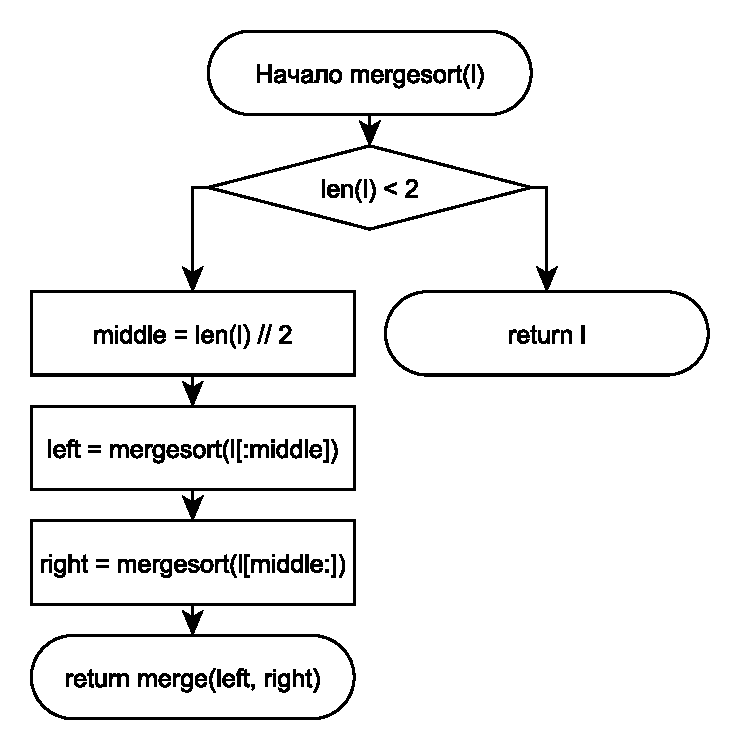
\includegraphics[width=\linewidth]{1.pdf}
%	\caption{Сортировка слиянием}
%	\label{graph2.1}
%\end{figure}

%\begin{figure}[h!]
%	\centering
%	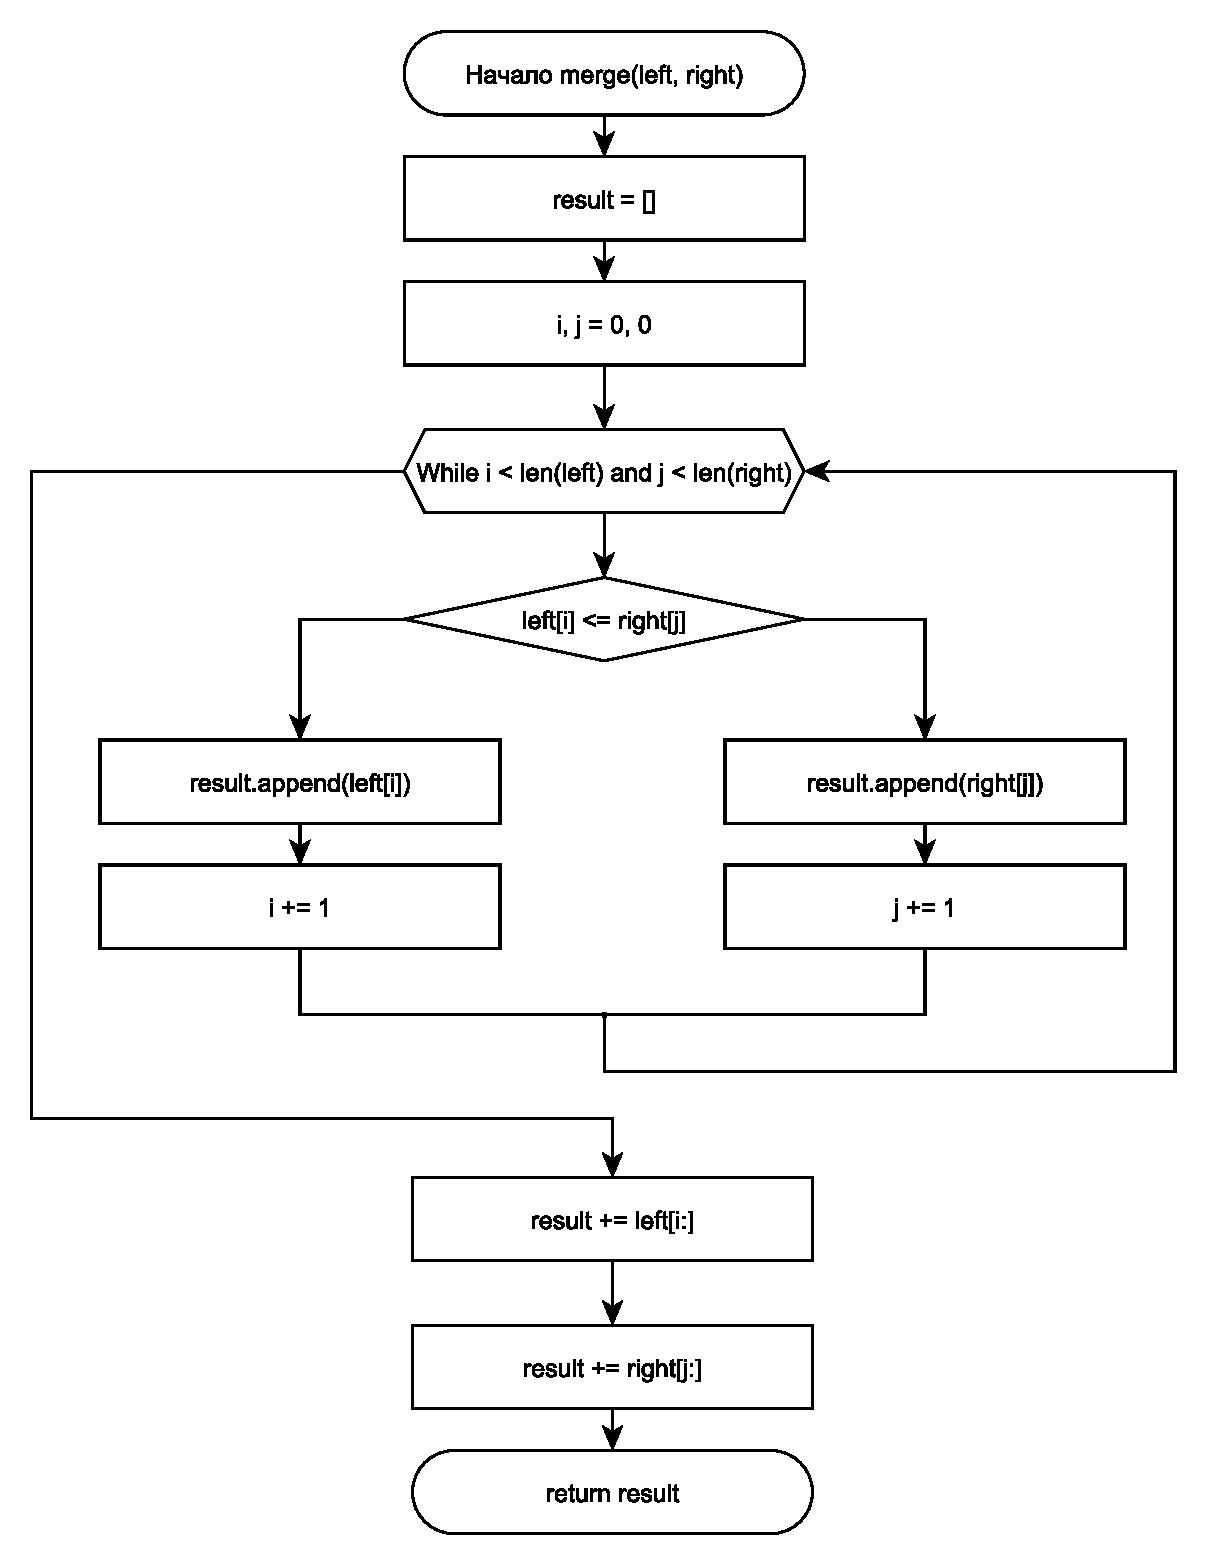
\includegraphics[width=\linewidth]{11.pdf}
%	\caption{Сортировка слиянием}
%	\label{graph2.2}
%\end{figure}

\begin{figure}[h!]
	\centering
	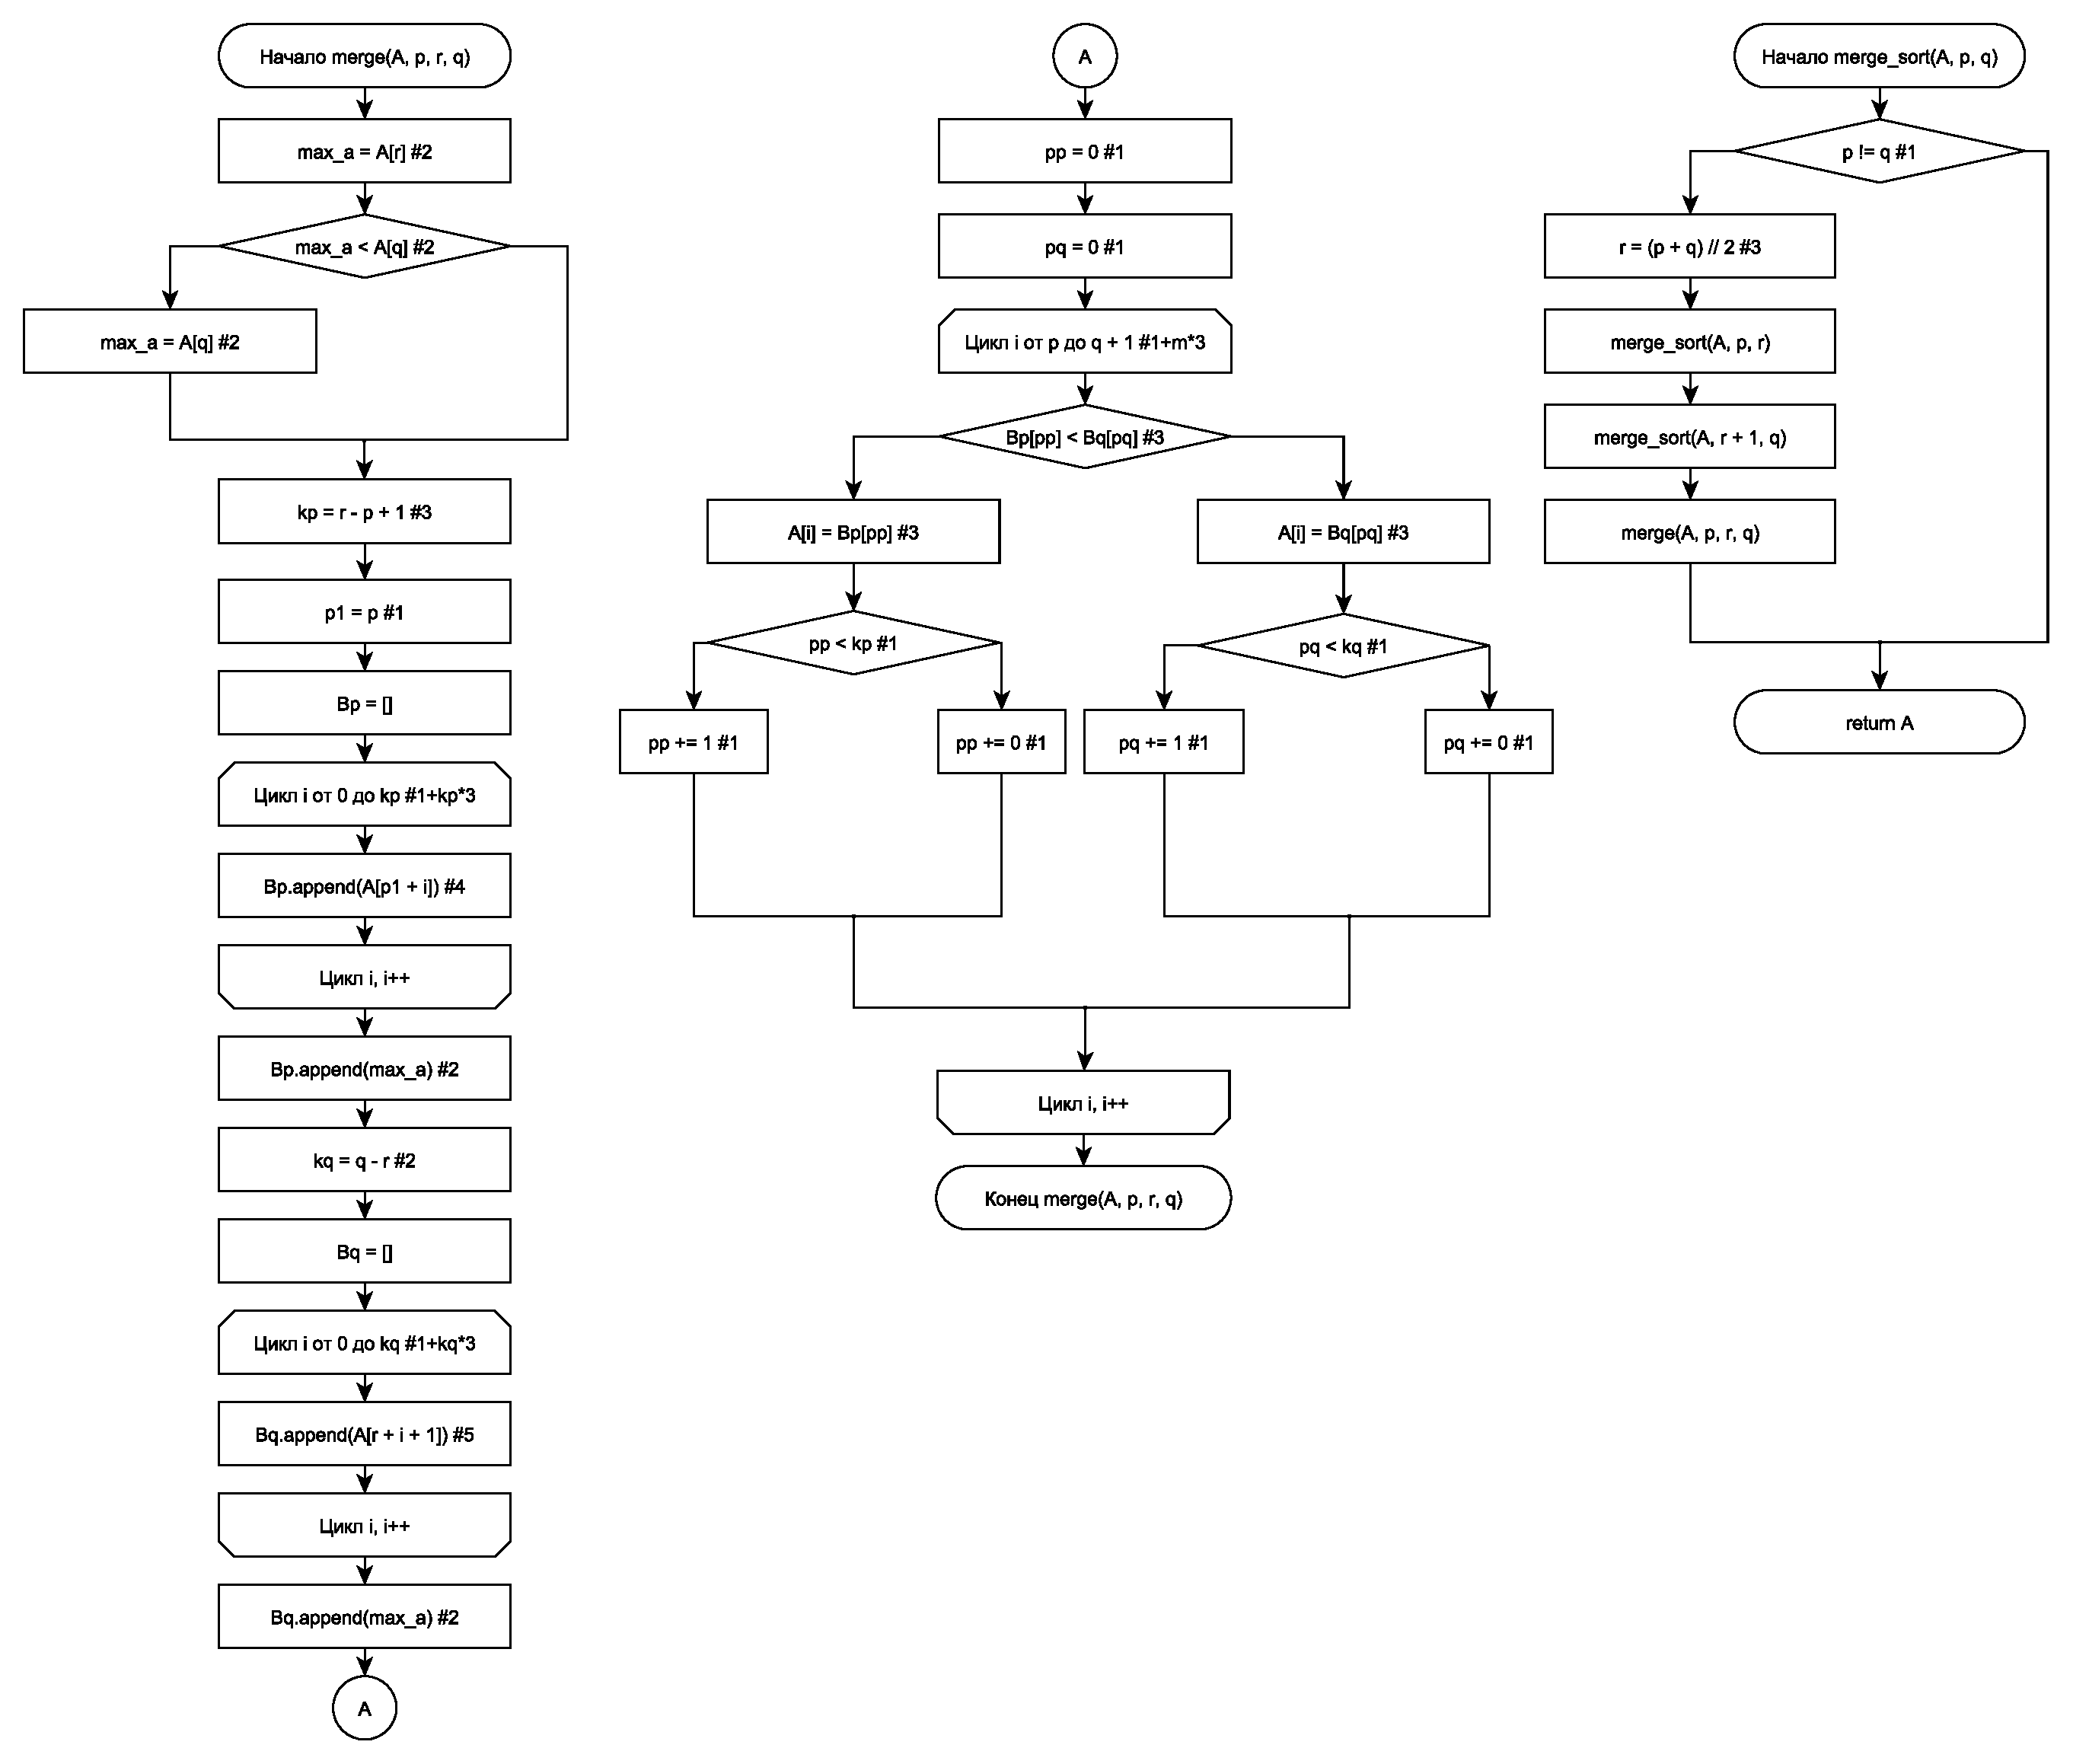
\includegraphics[width=\linewidth]{merge.pdf}
	\caption{Сортировка слиянием}
	\label{graph2.1}
\end{figure}

\begin{figure}[h!]
	\centering
	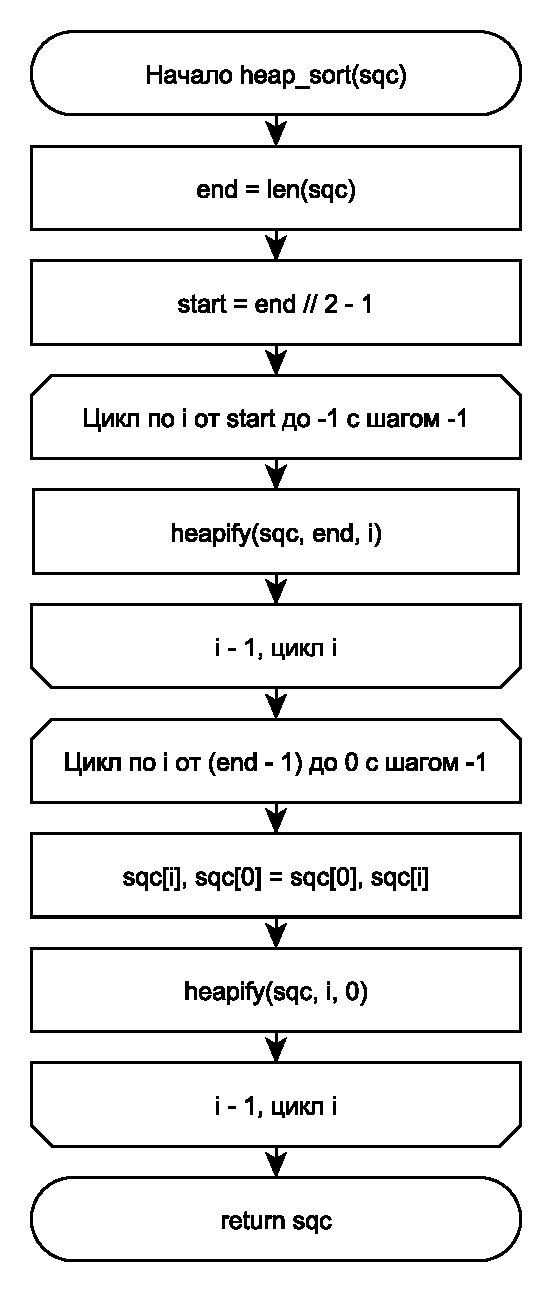
\includegraphics[width=200px]{2.pdf}
	\caption{Пирамидальная сортировка}
	\label{graph2.2}
\end{figure}

\begin{figure}[h!]
	\centering
	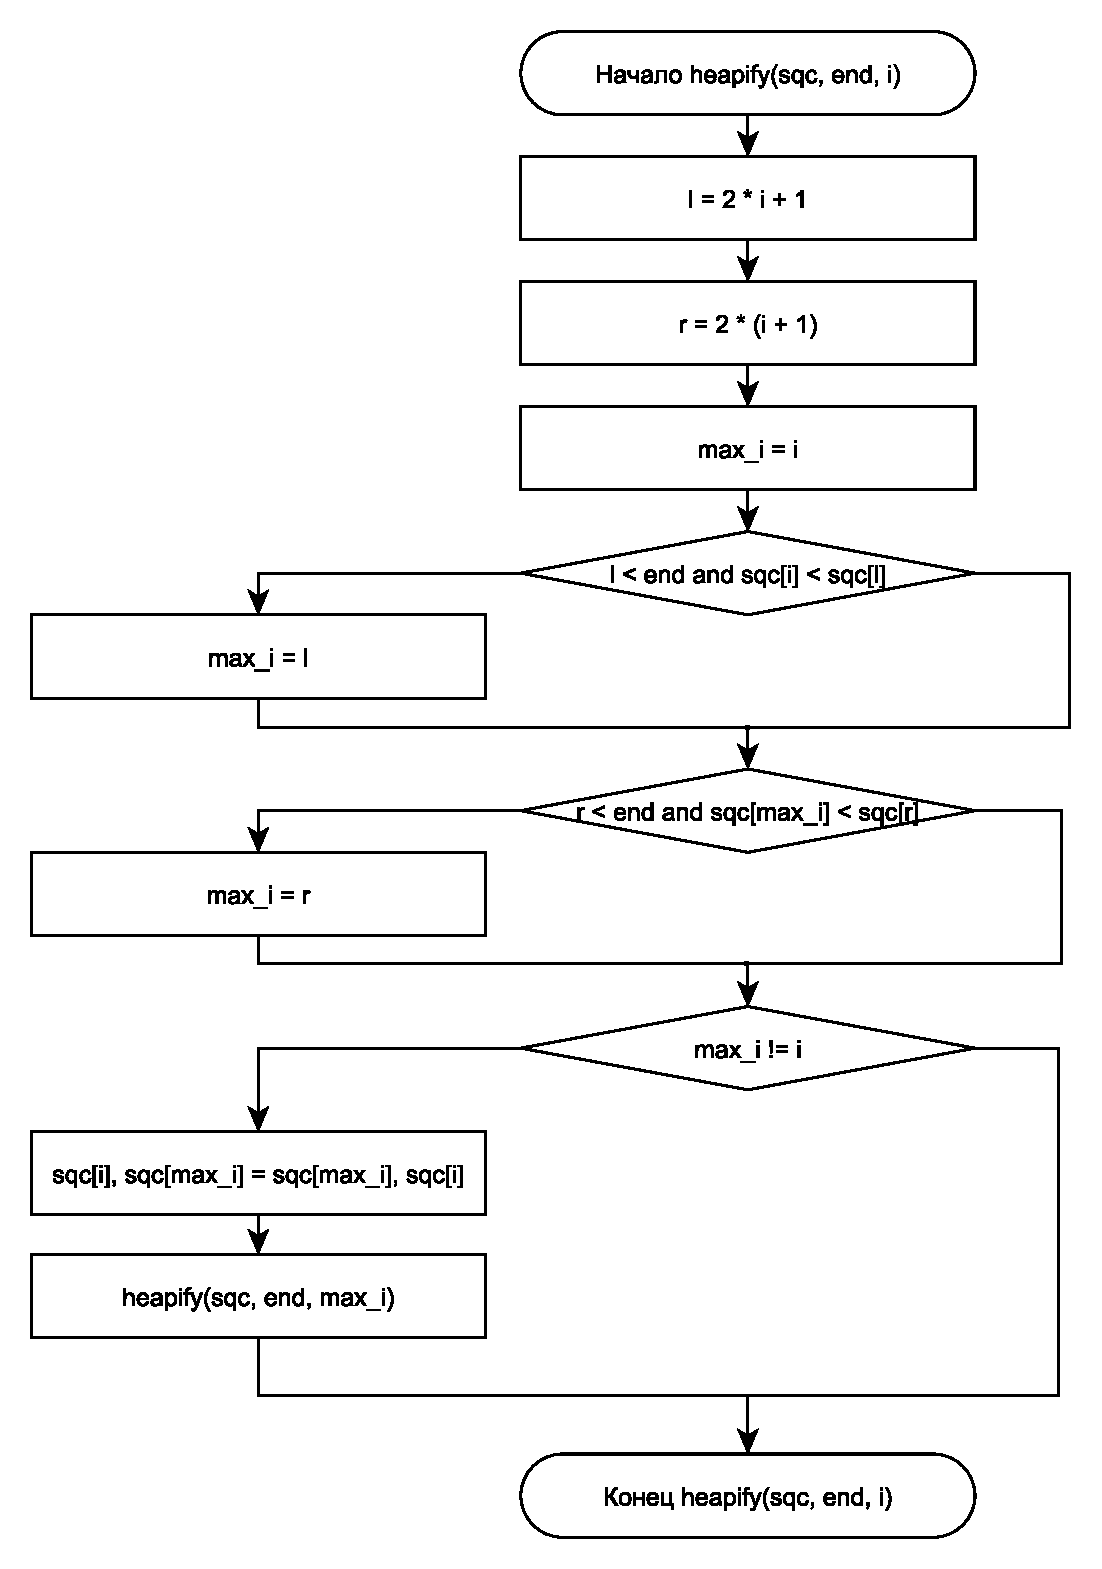
\includegraphics[width=300px]{21.pdf}
	\caption{Пирамидальная сортировка}
	\label{graph2.3}
\end{figure}

\begin{figure}[h!]
	\centering
	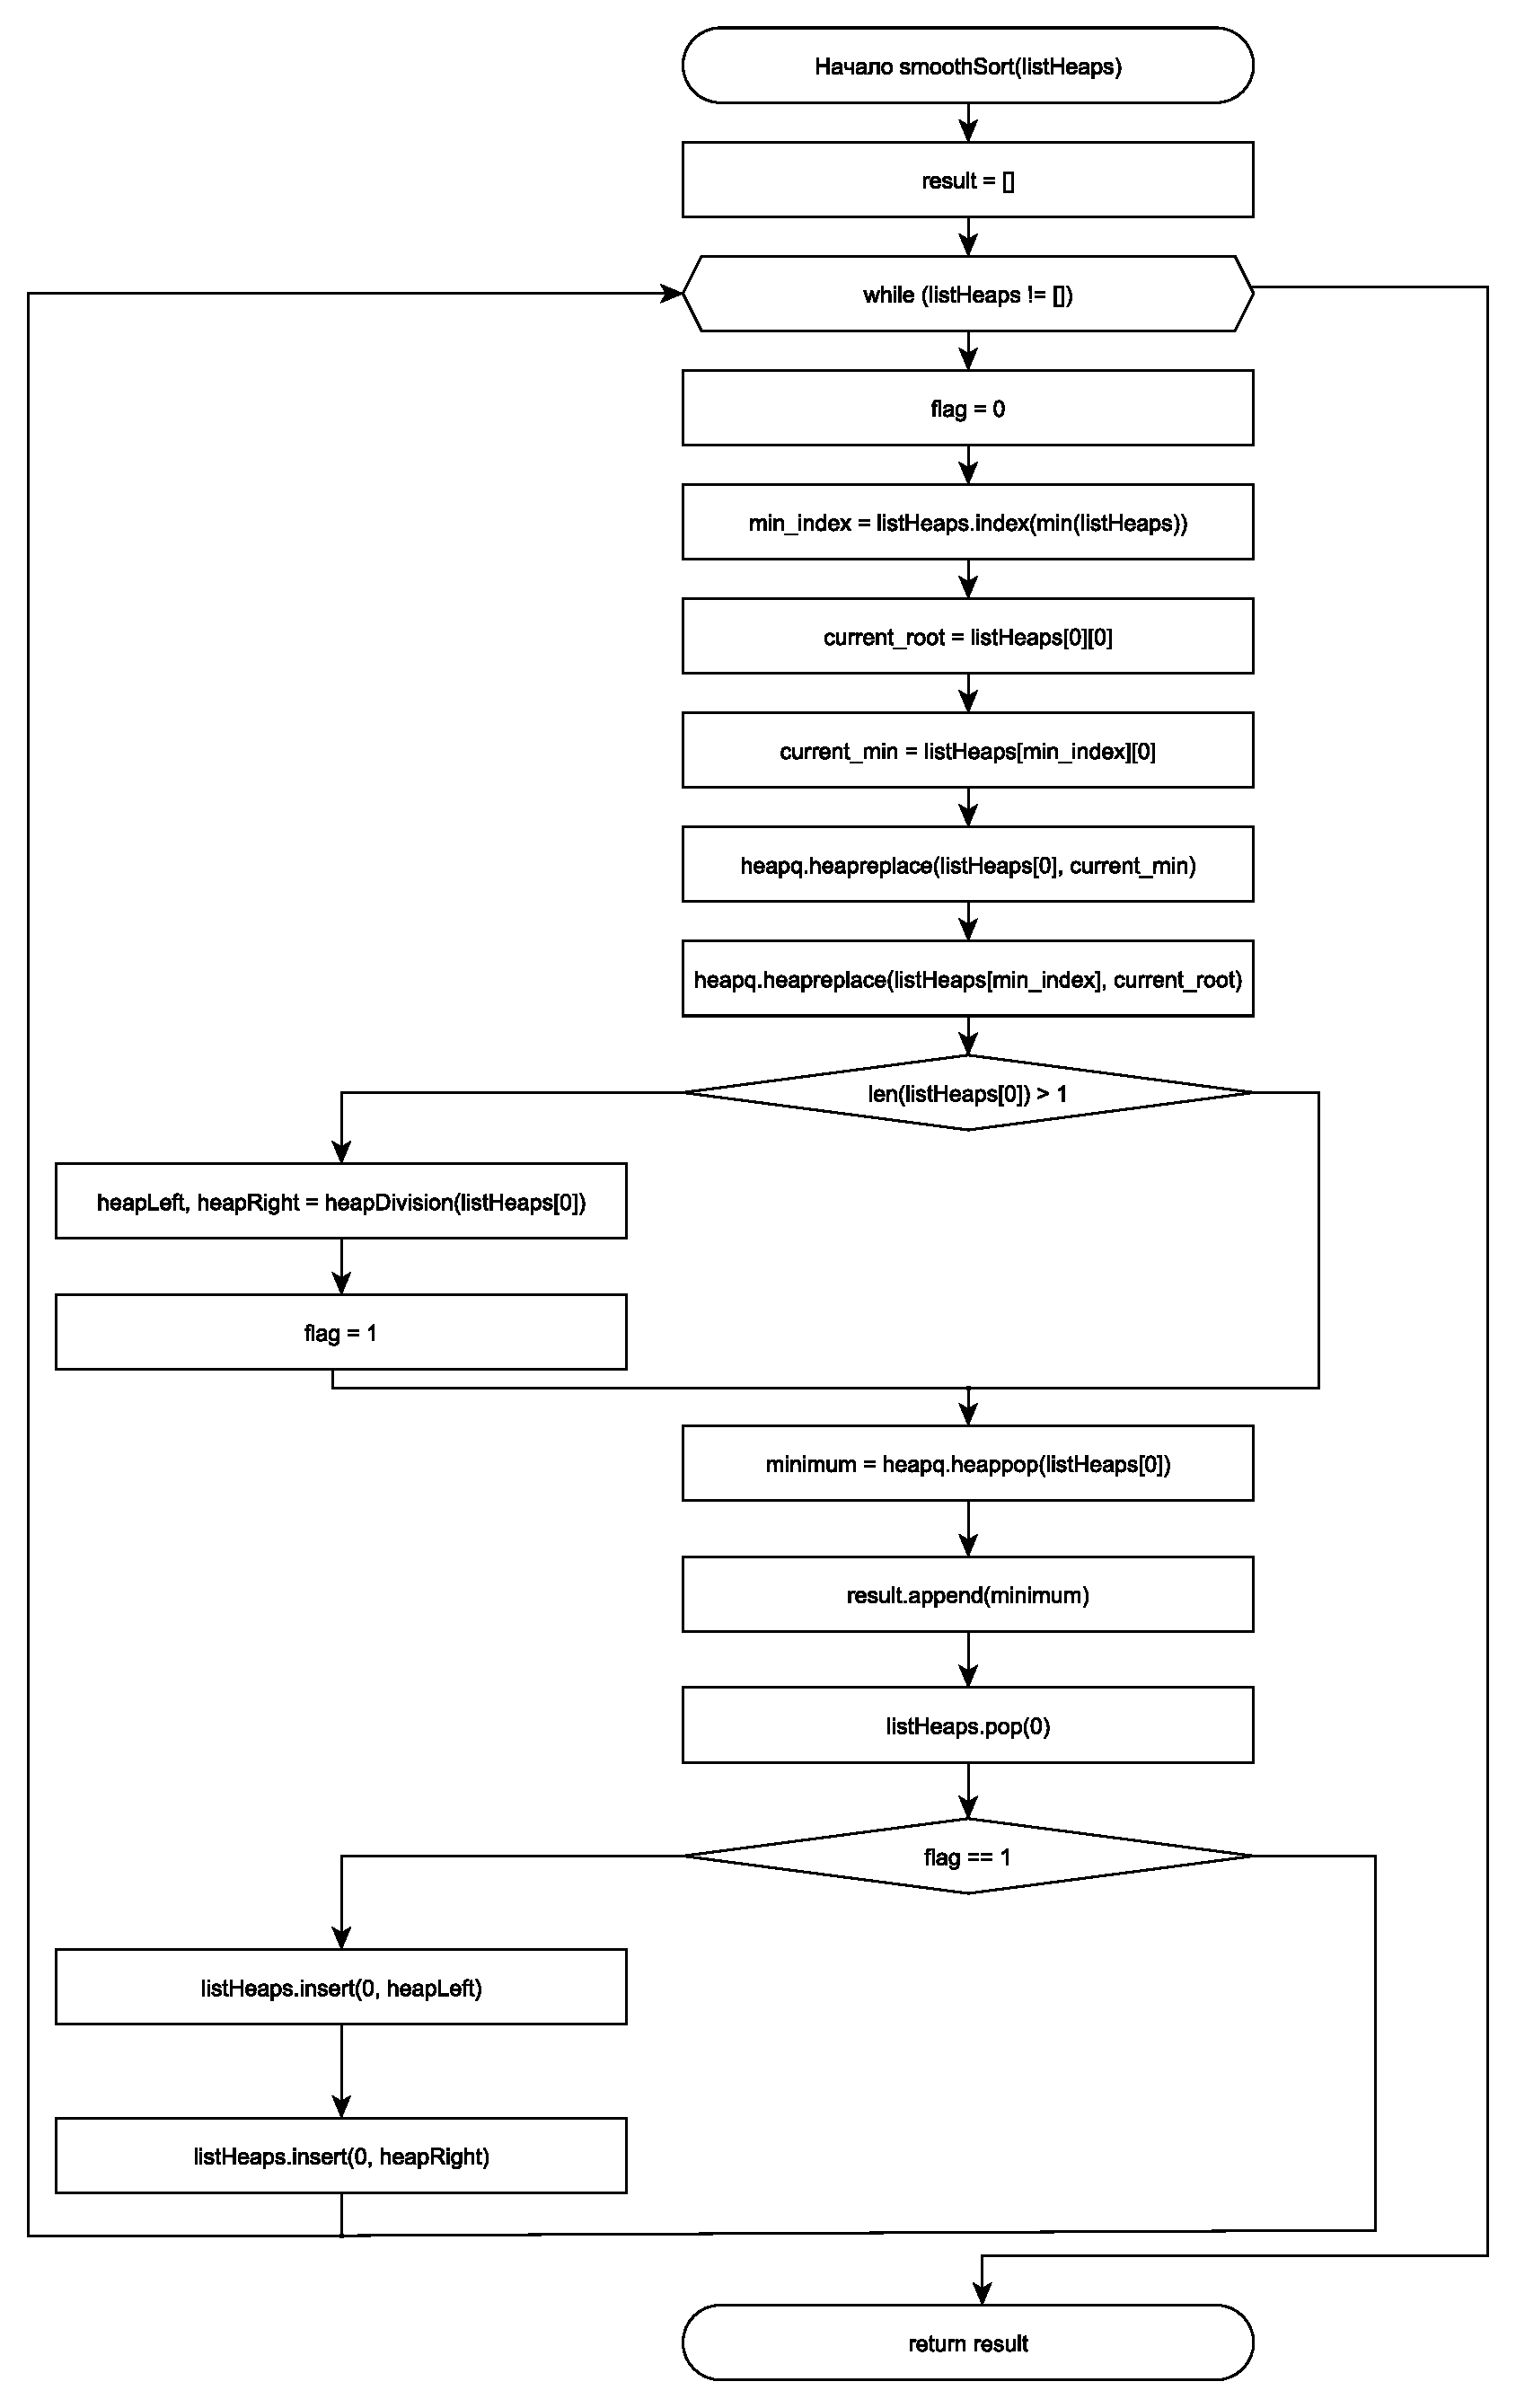
\includegraphics[width=400px]{3.pdf}
	\caption{Плавная сортировка}
	\label{graph2.4}
\end{figure}

\begin{figure}[h!]
	\centering
	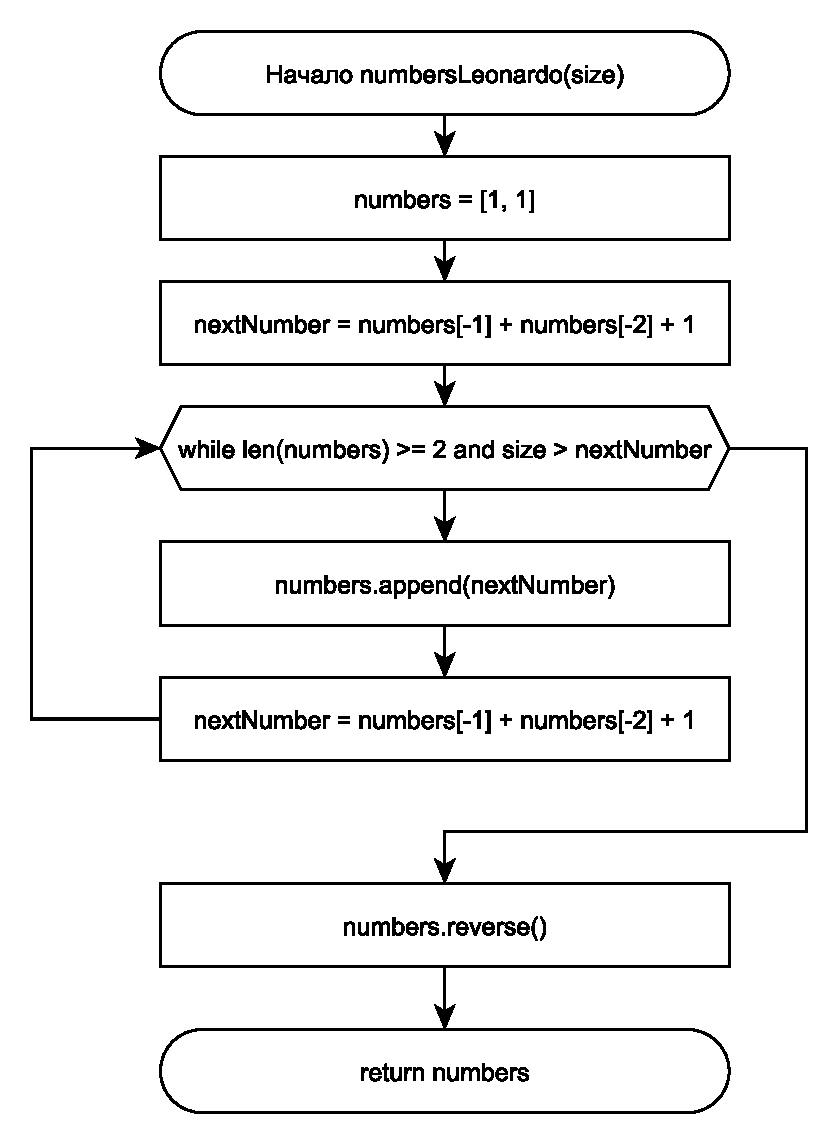
\includegraphics[width=300px]{31.pdf}
	\caption{Плавная сортировка}
	\label{graph2.5}
\end{figure}

\begin{figure}[h!]
	\centering
	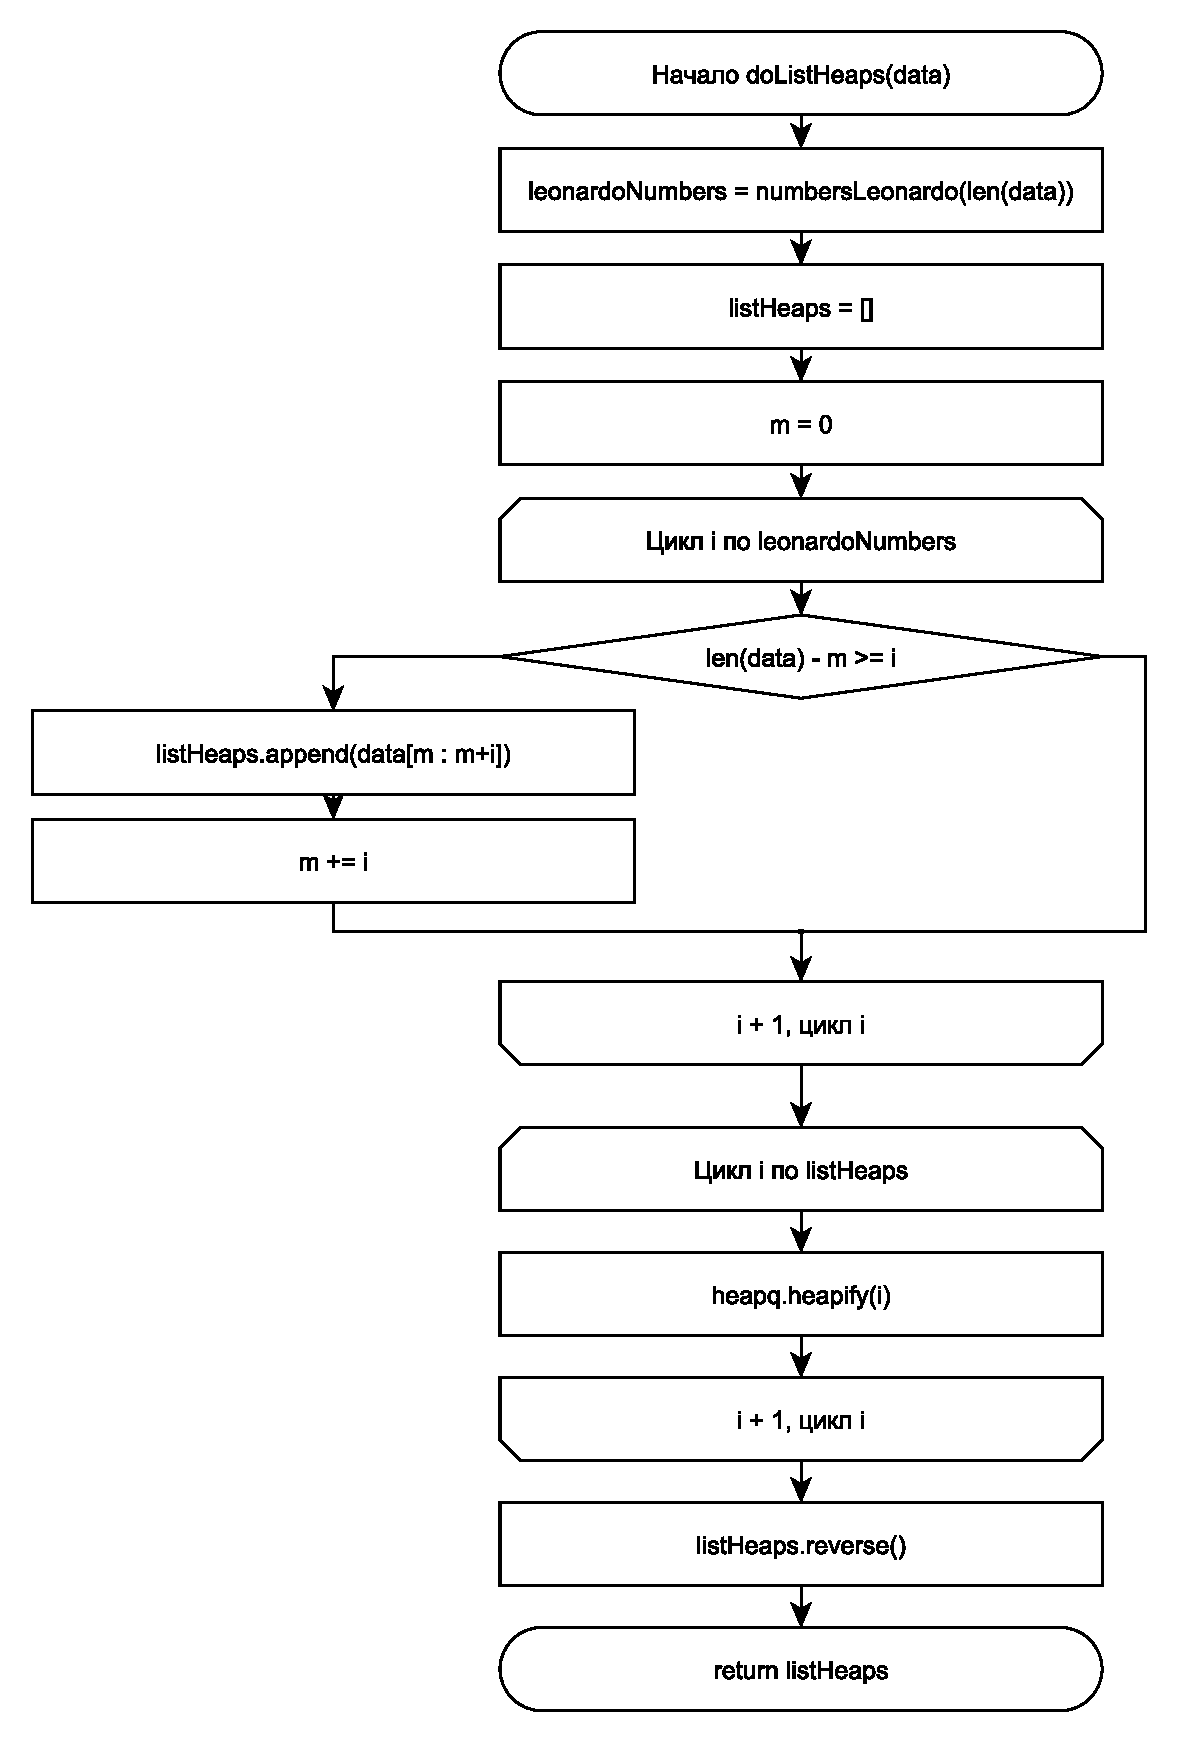
\includegraphics[width=300px]{32.pdf}
	\caption{Плавная сортировка}
	\label{graph2.6}
\end{figure}

\begin{figure}[h!]
	\centering
	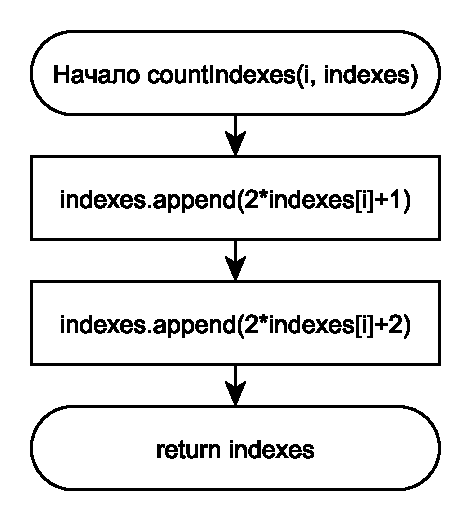
\includegraphics[width=300px]{33.pdf}
	\caption{Плавная сортировка}
	\label{graph2.7}
\end{figure}

\begin{figure}[h!]
	\centering
	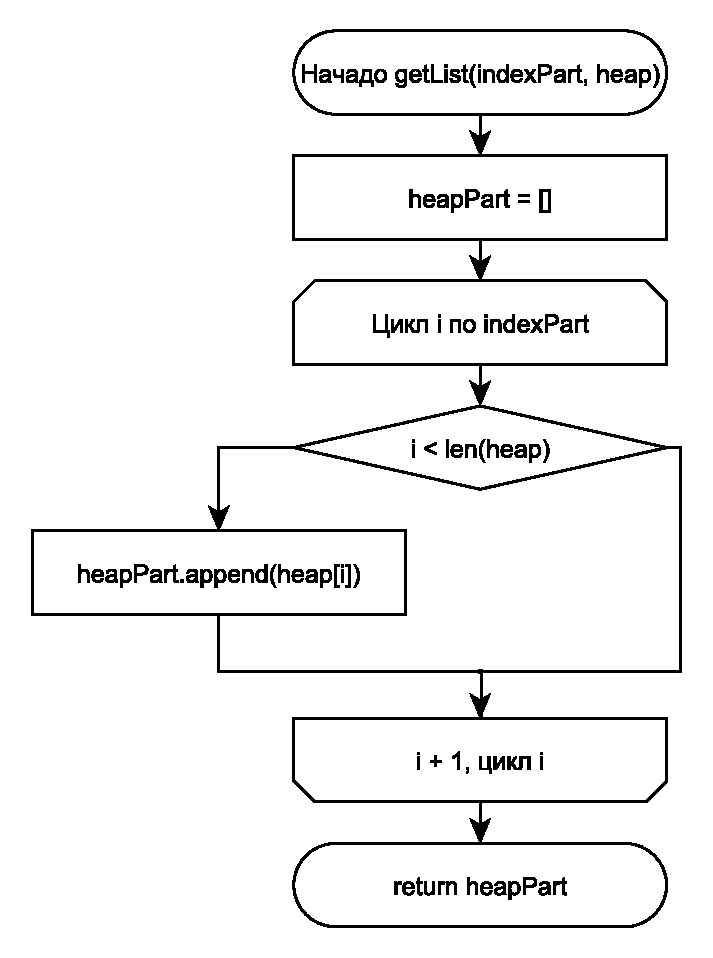
\includegraphics[width=300px]{34.pdf}
	\caption{Плавная сортировка}
	\label{graph2.8}
\end{figure}

\begin{figure}[h!]
	\centering
	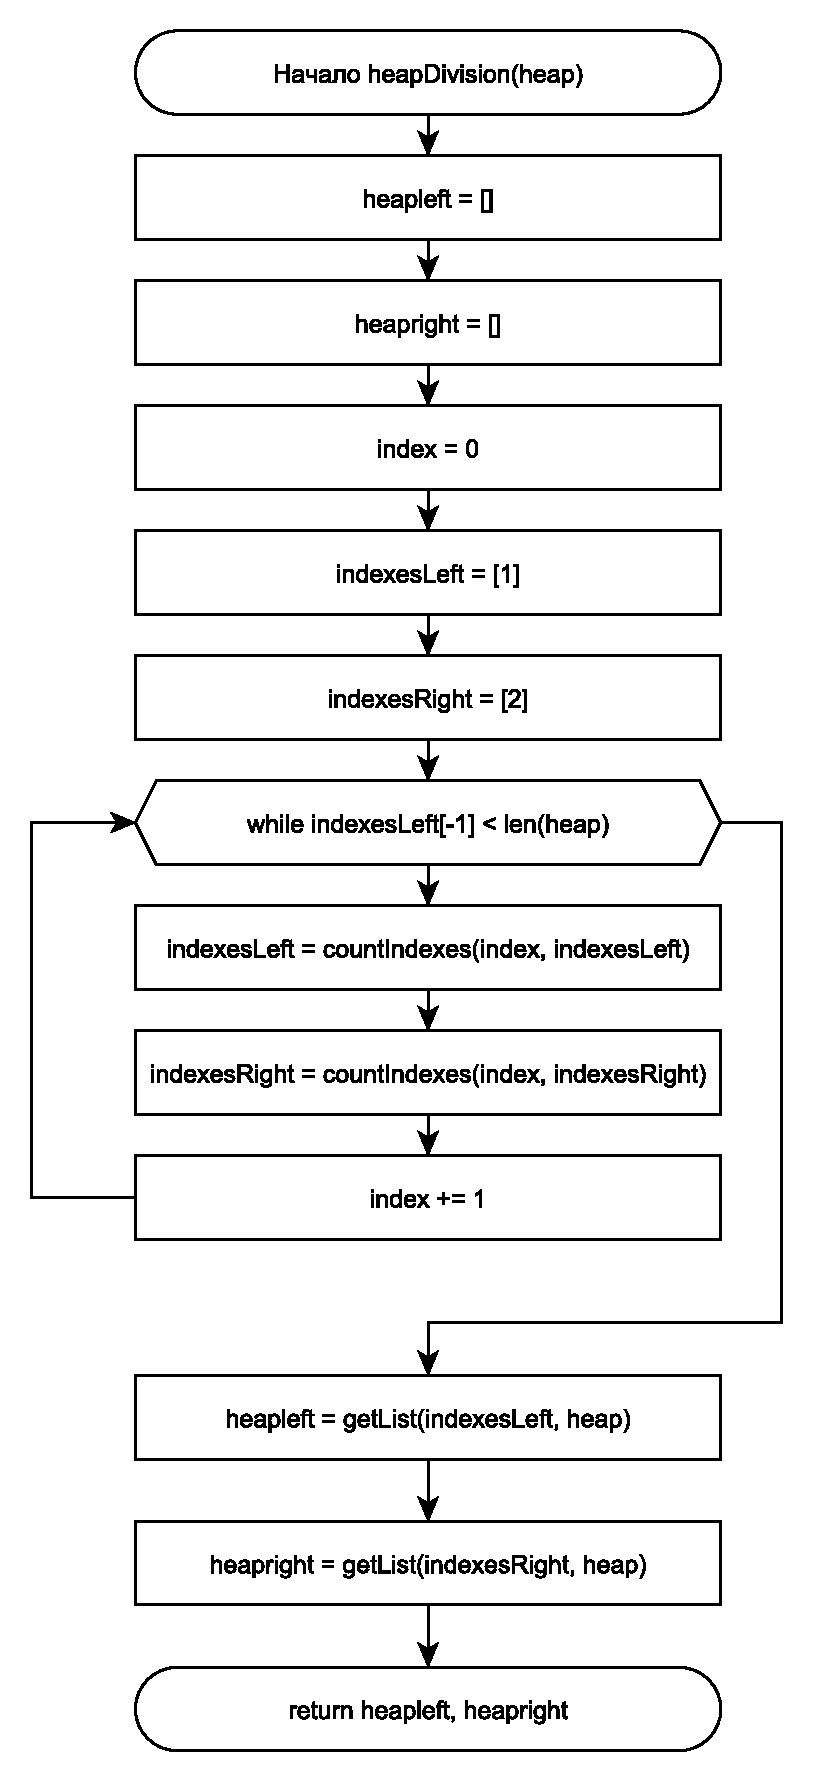
\includegraphics[width=300px]{35.pdf}
	\caption{Плавная сортировка}
	\label{graph2.9}
\end{figure}

Расчёт трудоёмкости алгоритма выполняется для алгоритма сортировки слиянием с использованием следующей модели трудоёмкости:\\
1) единичная трудоёмкость\\
$+$, $-$, $*$, $/$, $//$, остаток от деления, $<$, $<=$, $=>$, $>$, $==$, $=$, $!=$, $[]$, $+=$, $-=$, $*=$, $/=$, $++$, $--$, $.$, len(), взятие части связного списка (работа со срезами в ЯП Python); \\
2) цикл (C-подобная модель | Python) \\
for (int i = 0; i < N; i++) | for i in range(N) \\
COMP(цикла) = 2 + N*(2 + COMP(тела)) \\
for (int i = 0; i < N+1; i++) | for i in range(N+1) \\
COMP(цикла) = 3 + N*(3 + COMP(тела)) 

%Трудоёмкость вспомогательной функции merge, принимающей левый и правый подмассивы: \\
%Лучший и худший случаи данной функции непосредственно зависят от числа итераций цикла while. Длины подмассивов различаются не более чем на 1. \\
%Пусть сумма длин подмассивов равна N. Тогда лучший случай наступает в случае, когда число итераций цикла равно N//2, в то время как худший - (N-1).\\
%\begin{equation}\label{eq2.1}
%COMP(merge) = 1 + 2 + [N//2; N-1] * 6 + 2 + 2 = 7 + 6 * [N//2; N-1],  
%COMP(mergesort) = ?
%\end{equation}

Трудоёмкось алгоритма практически не зависит от данных. В блоке условия if Bp[pp] < Bq[pq] содержится одинаковое число операций, следовательно, выбор ветви не повлияет на трудоёмкость.
%\begin{equation}
%left[i] \leqslant right[j] 
%\end{equation}
%ветви содержат одинаковое число операций, следовательно, вероятность выбора той или иной ветви (что зависит от данных) не влияет на трудоёмкость конструкции ветвления в целом.

Трудоёмкость данного алгоритма для объединённого массива, имеющего длину 
\begin{equation*}
 m = k*p + k*q = q - p + 1.
\end{equation*}
Строка max\_a = A[q] выполняется в среднем для половины обращений.
Трудоёмкость алгоритма слияния отсортированных массивов как функция длины массива результата:
\begin{equation}\label{eq2.1}
f_{merge}^-(m) = 2 + 2 + 1 + 3 + 2 + 1 + 3*kp + 4*kp + 3 + 2 + 1 + 3*kq + 4*kq + 3 + 1 + 1 + 1 + 3*m + m*(3 + 5)
\end{equation}
\begin{equation}\label{eq2.2}
f_{merge}^-(m) = 11*m + 7*(kp + kq) + 23 = 18*m + 23
\end{equation}

Проведём анализ алгоритма методом подсчёта дерева рекурсий. Метод подсчёта дерева рекурсий - один из методов, применяемых для временной и ёмкостной трудоёмкости рекурсивных алгоритмов. Итоговая сумма базовых операций формируется с помощью вершин дерева рекурсии. Суммарные ресурсы, требуемые рекурсивной реализацией алгоритма, могут быть раздеены на ресурсы, собственно связанные с решением задачи, и ресурсы, необходимые для организации рекурсии. Если можно определить ресурсные затраты в каждой вершине дерева, то, суммируя, можно получить ресурсную функцию алгоритма в целом, что, собственно, и является методом подсчёта дерева рекурсии. Первым этапом такого подхода является исследование дерева рекурсии, на основе чего строятся функции-характеристики. \cite{Tree}

Случай 1. Длина массива - степень двойки. \\
Длина входа 
\begin{equation}\label{eq2.3}
n = 2^k, где k = log_2(n).
\end{equation}
Массив делится ровно пополам, после чего продолжает делиться рекурсивно до тех пор, пока в каждом подмассиве не останется по 1 элементу. В данном случае получается дерево рекурсий, которое представляет собой бинарное дерево глубины k, содержащиее числое листьев, равное n. 
\begin{figure}[h!]
	\centering
	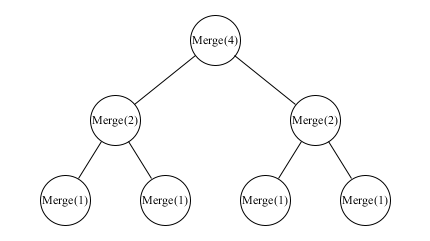
\includegraphics[width=\linewidth]{1.png}
	\caption{Бинарное дерево сортировки слиянием на примере массива длины 4}
	\label{graph2.11}
\end{figure}
Общее количество вершин подобного бинарно дерева R(n) задаётся с помощью формулы суммы геометрической прогрессии:
\begin{equation}\label{eq2.3}
R(n) = 1 + 2 + ... + 2^k = 2 * 2^k - 1 = 2*n - 1
\end{equation}
Поскольку полное бинарное дерево содержит 
\begin{equation}\label{eq2.4}
n = 2^k
\end{equation}
листьев, то 
\begin{equation}\label{eq2.5}
R_L(n) = n,
\end{equation}
количество внутренних вершин, порождающих рекурсию, равно
\begin{equation}\label{eq2.6}
R_v(n) = n - 1.
\end{equation}
Вызов данного алгоритма для сортировки массива длины n порождает дерево рекурсии со следующими характеристиками:
\begin{equation}\label{eq2.7}
R(n) = 2*n - 1, R_L(n) = n, R_v(n) = n - 1, H_R(n) = 1 + log_2(n), B_L(n) = R_L(n) / R(n) = n / (2*n - 1),
\end{equation}
где Hr(n) - высота, k - уровни, Rl(n) - количество листьев, Bl(n) - относительная ширина нижнего уровня в дереве рекукрсии.

Определим трудоёмкость функции merge\_sort(l) на один вызов fr(1) в соответствии  с методом подсчёта вершин дерева рекурсии. Функция имеет три параметра (p = 3), в стеке сохраняются значения четырёх регистров (r = 4), ни одно значение не возвращается через имя функции (f = 0), а функция имеет одну локальную переменную r (l = 1), то в результате получено:
\begin{equation}\label{eq2.8}
f_R(1) = 2*(3 + 4 + 0 + 1 + 1) = 18,
\end{equation}
следовательно, с учётом предыдущей формулы,
\begin{equation}\label{eq2.9}
f_R(n) = R(n)*f_R(1) = (2*n - 1)*18 = 36*n - 18.
\end{equation}
Трудоёмкость останова рекурсии включает в себя одно сравнение, таким образом 
\begin{equation*}
f_{CL}(1) = 1,
\end{equation*}
следовательно,
\begin{equation}\label{eq2.10}
f_{CL}(n) = R_L(n)*f_{CL}(1) = n*1 = n.
\end{equation}

Во всех внутренних вершинах дерева (фрагмент рекурсивного вызова) трудоёмкость включает в себя подготовку рекурсивного вызова, вызов и возврат функции 
\begin{equation*}
merge(A, p, r, q) - f_{merge\_sort}(v),
\end{equation*}
и трудоёмкость выполнения функции
\begin{equation*}
merge(A, p, r, q) - f_{merge}(v).
\end{equation*}
Трудоёкость во внутренней вершине fcv(v) и суммарную трудоёмкость внутренних вершин fcv(n) можно представить в виде следующих сумм:
\begin{equation}\label{eq2.11}
f_{CV}(v) = f_{merge\_sort}(v) + f_{merge}(v),
f_{CV}(n) = f_{CV merge\_sort}(n) + f_{CV merge}(n).
\end{equation}
Вычисление значения fmerge\_sort(v): выполняется сравнение, вычисление середины длины, прибавление единицы (r+1) и передача управления merge(A, p, r, q) с сохранением значения переменной r (l=1), после чего управление возвращается обратно, т.е.
\begin{equation}\label{eq2.12}
f_{merge\_sort}(v) = 1 + 3 + 1 + 2*(4 + 4 + 0 + 1 + 1) = 25.
\end{equation}
Сумма по всем внутренним вершинам:
\begin{equation}\label{eq2.13}
f_{CV mergesort}(n) = R_v(n)*f_{mergesort}(v) = (n-1)*25 = 25*n - 25.
\end{equation}
Введём функццию
\begin{equation}\label{eq2.14}
g(v_j) = f_{merge}(v_j),
\end{equation}
являющуюся трудоёмкостью слияния в вершине vj. Для рассматриваемого случая на фиксированном уровне рекурсивного дерева слиянию подвергаются массивы одинаковой длины. Поскольку одинаковые слагаемые, связанные одним уровнем, могут быть объединены:
\begin{equation}\label{eq2.15}
\sum \limits_{j=1}^{R_v(n)} g(v_j).
\end{equation}
Согласно формуле \label{eq2.1} , трудоёмкость алгоритма слияния для массива длины m составляет 
\begin{equation*}
18*m + 23,
\end{equation*}
причём алгоритм вызывается
\begin{equation*}
R_v(n) = n - 1
\end{equation*}
раз с разными длинами объединяемых фрагментов массива на каждом уровне дерева. Следовательно, значения g(vj) имеют вид
\begin{equation}\label{eq2.16}
\begin{matrix}
    g(v_j) & :
    & \left\{
    \begin{matrix}
    g(v_1) & = & 18*n + 23; \\
    g(v_2) & = & g(v_3) & = & 18*(n/2) + 23;\\
    g(v_4) & = & g(v_5) & = & g(v_6) & = & g(v_7) & = & 18*(n/4) + 23; \\
    ...
    \end{matrix} \right.
    \end{matrix}
\end{equation}

В результате суммирования g по всем внутренним вершинами дерева:
\begin{equation}\label{eq2.17}
f_{CV merge}(n) = \sum \limits_{j=1}^{R_v(n)} g(v_j) = 23*R_v(n) + 18*n + 2*18*(n/2) + 4*18*(n/4) + ... .
\end{equation}
Учитывая, что таким образом обрабатываются все уровни дерева, кроме последнего, который не содержит внутренних вершин, т.е. k уровней рекурсивного дерева с номерами от 0 до k - 1, получаем:
\begin{equation}\label{eq2.18}
f_{CV merge}(n) = 18*n*k + 23*(n - 1) = 18*n*log_2(n) + 23*n - 23.
\end{equation}

Окончательный вид функции трудоёмкости для алгоритма сортировки слиянием в случае 
\begin{equation*}
n = 2^k
\end{equation*}
будет выглядеть следующим образом:
\begin{equation}\label{eq2.18}
f_A^-(n) = f_R(n) + f_{CL}(n) + f_{CV merge\_sort}(n) + f_{CV merge}(n)
\end{equation}
\begin{equation}\label{eq2.19}
f_A^-(n) = 36*n - 18 + n + 25*n - 25 + 18*n*log_2(n) + 23*n - 23 = 18*n*log_2(n) + 85*n - 66.
\end{equation}
Доля операций обслуживания дерева рекурсии составляет
\begin{equation}\label{eq2.20}
F_R(n) = f_R(n) / f_A(n) = (36*n - 18) / (18*n*log_2(n) + 85*n - 66).
\end{equation}
Значения 
\begin{equation*} 
F_R(n) 
\end{equation*} 
медленно убывают с ростом длины массива.

Функция трудоёмкости в среднем 
\begin{equation*}
f_A^-(n)
\end{equation*}
по реультату оценки главного порядка обладает сложностью 
\begin{equation}\label{eq2.21}
O(n*log_2(n)).
\end{equation}
Такой же сложностью обладают и лучший и худший случаи. Они могут быть оценены исходя из того, что каждый вызов функции слияния при вычислении заглушки либо выполняет, либо пропускает две операции. Слияние выполняется для каждой внутренней вершины дерева.

Лучший случай:
\begin{equation}\label{eq2.22}
f_A^{best}(n) =  18*n*log_2(n) + 84*n - 67.
\end{equation}

Худший случай:
\begin{equation}\label{eq2.22}
f_A^{worst}(n) =  18*n*log_2(n) + 86*n - 65.
\end{equation}

Случай 2. Длина входа 
\begin{equation*}
2^{k-1} < n < 2^k, k = |log_2(n)|.
\end{equation*}
Алгоритм получает на входе массив из n элементов, делит его на две равные части при чётном n или на части, отличающиеся на единицу, при нечётном n. Деление продолжается рекурсивно до тех пор, пока алгоритм не дойдёт до единичных элементов массива. В результате работы алгоритма получается бинарное дерево рекурсий, содержащее k уровней, из которых только k - 1 уровней являются полными.
\begin{figure}[h!]
	\centering
	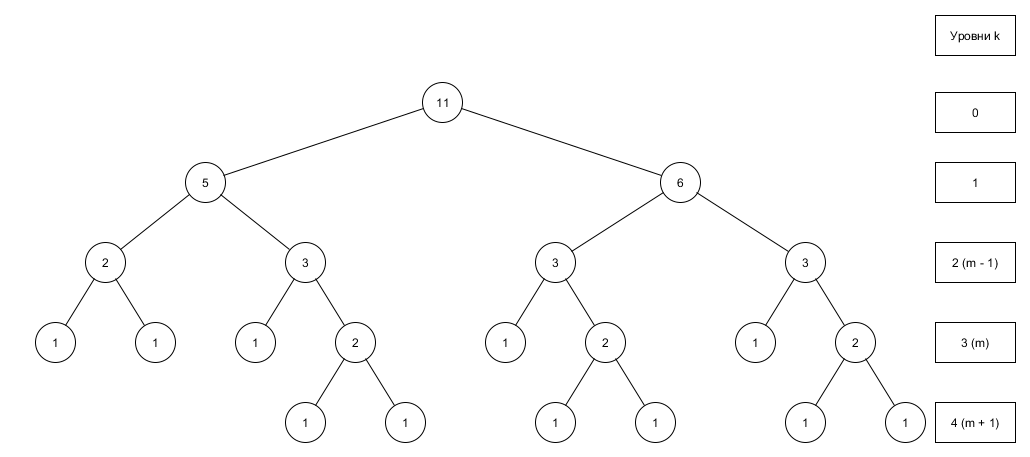
\includegraphics[width=\linewidth]{2.png}
	\caption{Бинарное дерево сортировки слиянием на примере массива длины 11}
	\label{graph2.12}
\end{figure}
Данное неполное дерево можно охарактеризовать следующими формулами, совпадающими с формулами для полного дерева:
\begin{equation}\label{eq2.23}
R(n) = 2*n - 1, R_L(n) = n, R_v(n) = n - 1, H_R(n) = 1 + log_2(n), B_L(n) = n / (2*n - 1),
\end{equation}
Поскольку формулы для характеристик дерева не изменились, связанные с ним формулы трудоёмкости компонентов остаются в силе. Изменения в случае 2 касаются трудоёмкости слияния во внутренних вершинах
\begin{equation}\label{eq2.24}
f_{CV merge}(n) = \sum \limits_{j=1}^{R_v(n)} g(v_j)
\end{equation}
Введём нумерацию внутренних вершин по уровням дерева и обозначим через
\begin{equation*}
(n_j)^k
\end{equation*}
длину фрагмента массива, обрабатываемого в j-ой внутренней вершине k-го уровня, а через
\begin{equation*}
(v_j)^k
\end{equation*}
обозначим саму эту вершину. С учётом того, что
\begin{equation}\label{eq2.25}
g((v_j)^k) = 18*n_j^k + 23,
\end{equation}
искомая сумма может быть записана следующим образом:
\begin{equation}\label{eq2.26}
f_{CV merge} (n) = \sum \limits_{j=1}^{R_v(n)} (18*n_j^k + 23) = 23*R_v(n) +  \sum \limits_{j=1}^{R_v(n)} 18*n_j^k.
\end{equation}
Дерево рекурсии является полным, за исключением последнего уровня. Пусть
\begin{equation}\label{eq2.27}
m = log_2(n)
\end{equation}
является номером последнего полного уровня, тогда предыдущий уровень m - 1 не содержит листьев, а последний (m + 1)-й уровень содержит только листья. На уровне m могут находиться как листья, так и внутренние вершины. Поскольку дерево является бинарным, а на уровне m + 1 находятся только листья, то 
\begin{equation*}
(n_j)^m = 2.
\end{equation*}
Поскольку увеличение n на единицу приводит к созданию новой внутренней вершины, а для полного бинарного дерева все вершины последнего уровня являются листьями, то на уровне m будет находиться
\begin{equation*}
n - 2^m
\end{equation*}
внутренних вершин. Исходя из этого, мы можем переписать формулу для 
\begin{equation*}
f_{CV merge}(n)
\end{equation*}
в виде двух сумм: суммы по всем m - 1 уровням, содержащим только внутренние вершины, и суммы по внутренним вершинам уровня m:
\begin{equation}\label{eq2.28}
 \sum \limits_{j=1}^{R_v(n)} 18*n_j^k = \sum \limits_{k=0}^{m-1} \sum \limits_{j=1}^{2^k} 18*n_j^k + \sum \limits_{j=1}^{n-2^m} 18*n_j^m.
\end{equation}
Поскольку сумма объединённых фрагментов массива на полных уровнях рекурсивного дерева всегда равна полной длине массива n, а
\begin{equation*}
(n_j)^m = 2,
\end{equation*}
то
\begin{equation}\label{eq2.29}
 \sum \limits_{j=1}^{R_v(n)} 18*n_j^k = 18*n*m + 18*(n - 2^m) *2.
\end{equation}
\begin{equation}\label{eq2.30}
f_{CV merge}(n) = 23*R_v(n) + 18*n*m + 18*(n - 2^m)*2
\end{equation}
Поскольку
\begin{equation*}
m = log_2(n), R_v(n) = n - 1,
\end{equation*}
то
\begin{equation}\label{eq2.31}
f_{CV merge}(n) = 18*n*log_2(n) + 59*n - 36*2^{log_2(n)} - 23.
\end{equation}

Трудоёмкость алгоритма сортировки в среднем для случая, где длина массива не равна степеням двойки:
\begin{equation}\label{eq2.32}
f_A^-(n) = f_R(n) + f_{CL}(n) + f_{CV merge\_sort}(n) + f_{CV merge}(n)
\end{equation}
\begin{equation}\label{eq2.33}
f_A^-(n) = 36*n - 18 + n + 25*n - 25 + f_{CV merge}(n) = 18*n*log_2(n) + 121*n - 36*2^{log_2(n)} - 66.
\end{equation}
Как и в случае 1, разница между полученной трудоёмкостью в среднем и худшем и лучшем случаями равна n - 1.

Аналогично случаю 1, по реультату оценки главного порядка трудоёмкости среднего, лучшего и худшего случаев обладают сложностью 
\begin{equation}\label{eq2.34}
O(n*log_2(n)).
\end{equation}

\newpage
\section{Технологическая часть}

В данном разделе представлены средства реализации задачи и листинг кода.

\subsection{Требования к программному обеспечению}
Программа должна сортировать заданный массив одним из следующих методов:
\begin{enumerate}
	\item сортировка слиянием;
	\item пирамидальная сортировка;
	\item плавная сортировка.
\end{enumerate}

В программе должен быть реализован замер времени работы каждой сортировки на выборке размера 100..1000 для отсортированных значений, обратно отсортированных и для случайной выборки (средние значения 10 замеров сортировок на каждой выборке записываются в файлы для всех алгоритмов сортировки). Замеры производились для массивов со случайной выборкой элементов.

Минимальные системные требования: PC с операционной системой Windows версии XP/Vista/7/8/10. Требуются устройства ввода: клавиатура, мышь. 

\subsection{Средства реализации}

Для выполнения данной лабораторной работы был выбран язык программирования (ЯП) Python (3) ввиду его простоты и наглядности. Замеры времени производились посредством возможностей модуля time ЯП Python, в частности, с помощью perf\_counter.

Для генерации тестовых данных на массивах выборки 1000..10000 в данной лабораторной работе используются возможности модуля ЯП random, в частности, с помощью randint.



\subsection{Листинг кода}   
Программа сортировки слиянием $(merge\_sort.py):$

\begin{verbatim}
def merge(left, right):
    result = []
    i, j = 0, 0
    while i < len(left) and j < len(right):
        if left[i] <= right[j]:
            result.append(left[i])
            i += 1
        else:
            result.append(right[j])
            j += 1
    result += left[i:]
    result += right[j:]
    return result

# сортировка слиянием
# l - массив
def mergesort(l):
    if len(l) < 2:
        return l
    middle = len(l) // 2
    left = mergesort(l[:middle])
    right = mergesort(l[middle:])
    return merge(left, right)

#print(mergesort([9, 3, 1, 0, 2]))
\end{verbatim}

\begin{verbatim}
#A - массив, p, r, q - индексы 
#Bp, Bq - дополнительные массивы, куда выполняется
# копирование отсортированных частей
# Алгоритм слияния (Merge) отсортированных фрагментов массива A, 
# расположенных в позициях между (p и r) и (r+1 и q).
# Алгоритм использует доп.массивы, 
# в конец которых помещаются заглушки.
# Сначала выполняется копирование отсортированных 
# частей в Bp и Bq,
# затем объединённый массив формируется непосредственно 
# в массиве A между индексами p и q.

def merge(A, p, r, q):
    # формирование заглушки
    max_a = A[r]
    if max_a < A[q]:
        max_a = A[q]
    
    # копирование в массивы Bp, Bq    
    kp = r - p + 1
    p1 = p
    
    Bp = []
    for i in range(kp):
        Bp.append(A[p1 + i])
    Bp.append(max_a) #заглушка
    
    kq = q - r
    
    Bq = []
    for i in range(kq):
        Bq.append(A[r + i + 1])
    Bq.append(max_a) #заглушка
    
    # слияние частей
    pp = 0
    pq = 0 #инициализация указателей
    for i in range(p, q + 1):
        if Bp[pp] < Bq[pq]:
            A[i] = Bp[pp]
            pp += 1 if pp < kp else 0
        else:
            A[i] = Bq[pq]
            pq += 1 if pq < kq else 0
        
def merge_sort(A, p, q):
    if p != q:
        r = (p + q) // 2
        merge_sort(A, p, r)
        merge_sort(A, r + 1, q)
        
        merge(A, p, r, q)
    
    return A
\end{verbatim}

Программа пирамидальной сортировки $(heap\_sort.py):$

\begin{verbatim}
def heapify(sqc, end, i):   
    l = 2 * i + 1  
    r = 2 * (i + 1)   
    max_i = i   
    if l < end and sqc[i] < sqc[l]:   
        max_i = l   
    if r < end and sqc[max_i] < sqc[r]:   
        max_i = r   
    if max_i != i:
        sqc[i], sqc[max_i] = sqc[max_i], sqc[i]
        heapify(sqc, end, max_i)   

# пирамидальная сортировка
# sqc - массив
def heap_sort(sqc):     
    end = len(sqc)   
    start = end // 2 - 1
    for i in range(start, -1, -1):   
        heapify(sqc, end, i)   
    for i in range(end - 1, 0, -1):   
        sqc[i], sqc[0] = sqc[0], sqc[i]
        heapify(sqc, i, 0)

    return sqc

#sqc = [2, 7, 1, -2, 56, 5, 3]
#print(heap_sort(sqc[:]))
#print(sqc)
\end{verbatim}

Программа плавной сортировки $(smooth\_sort.py):$

\begin{verbatim}
import heapq

# формирование списка чисел Леонардо, являющихся размерами куч
# size - размер входного массива для плавной сортировки
# возвращает список чисел Леонардо
def numbersLeonardo(size):
    numbers = [1, 1] # начальные элементы для последовательности чисел Леонардо
    nextNumber = numbers[-1] + numbers[-2] + 1
    while len(numbers) >= 2 and size > nextNumber:
        numbers.append(nextNumber)
        nextNumber = numbers[-1] + numbers[-2] + 1
    numbers.reverse()
    return numbers

# формирование списка куч по числам Леонардо
# data - входной массив данных
# возвращает выходной список с кучами
def doListHeaps(data):
    # формируем список чисел Леонардо для входной последовательности
    leonardoNumbers = numbersLeonardo(len(data))
    # формируем список куч
    listHeaps = [] # финальный список куч
    m = 0 # хвост предыдущей части и начало следующей
    for i in leonardoNumbers:
        if len(data) - m >= i:
            # если оставшаяся нераспределённая часть входного массива данных 
	    # больше или равна очередному числу Леонардо
            listHeaps.append(data[m : m+i])
            # переходим к оставшейся нераспределённой части
            m += i
    # восстанавливаем свойство кучи для каждой кучи
    for i in listHeaps:
        heapq.heapify(i)
    # так как кучи неубывающие, конечный результат будет заполняться 
    # с начала - минимального элемента 
    # до максимального элемента последовательности, то меняем порядок 
    # куч на обратный
    listHeaps.reverse()
    return listHeaps

# формирование списка элементов по заданным индексам:
# i - индекс, потомки которого ищутся
# indexes - список индексов
def countIndexes(i, indexes):
    indexes.append(2*indexes[i]+1)
    indexes.append(2*indexes[i]+2)

    return indexes

# формирование подкучи из заданного списка индексов и исходной кучи
# indexPart - список индексов
# heapPart - найденная подкуча
def getList(indexPart, heap):
    heapPart = []
    for i in indexPart:
        if i < len(heap):
            heapPart.append(heap[i])

    return heapPart

# деление кучи на левые и правые подкучи
# heap - куча для деления
# возвращается кортеж из левой и правой подкучи
def heapDivision(heap):
    heapleft = []
    heapright = []
    index = 0
    indexesLeft = [1] # список индексов для элементов левой подкучи
    indexesRight = [2] # список индексов для элементов правой подкучи
    while indexesLeft[-1] < len(heap): 
        # исходя из логики построения куч, левая подкуча никогда не будет 
        # меньше правой

        # считаем индексы для левой подкучи
        indexesLeft = countIndexes(index, indexesLeft)

        # считаем индексы для правой подкучи
        indexesRight = countIndexes(index, indexesRight)

        index += 1

    # составляем списки левой и правой подкуч
    heapleft = getList(indexesLeft, heap)
    heapright = getList(indexesRight, heap)

    return heapleft, heapright

# плавная сортировка
# listHeaps - кучи
# возвращает отсортированную последовательность данных
def smoothSort(listHeaps):
    result = []
    while (listHeaps != []):
        # чтобы не писать пустые подкучи
        flag = 0
        # находим минимальный элемент среди корней куч
        min_index = listHeaps.index(min(listHeaps)) # индекс кучи
        # с минимальным корнем
        # меняем его местами с корнем первой кучи
        # запомним корень текущей кучи
        current_root = listHeaps[0][0]
        # и минимальный элемент
        current_min = listHeaps[min_index][0]
        heapq.heapreplace(listHeaps[0], current_min)
        heapq.heapreplace(listHeaps[min_index], current_root)
        # т.к. корень первой кучи будет в дальнейшем удален, размер кучи
        # уменьшится на 1 -> образуются две кучи из его левого и 
        # правого поддерева
        if len(listHeaps[0]) > 1:
            heapLeft, heapRight = heapDivision(listHeaps[0])
            flag = 1
        # удаляем корень первой кучи - это минимальный элемент 
        # из всех возможных
        minimum = heapq.heappop(listHeaps[0])
        # ставим его в конечную последовательность чисел
        result.append(minimum)
        # удалим первый элемент списка и вставим его ранее 
        # полученные поддеревья
        listHeaps.pop(0)
        # добавим две получившиеся кучи в начало всей 
        # последовательности куч
        if flag == 1:
            listHeaps.insert(0, heapLeft)
            listHeaps.insert(0, heapRight)
    return result

#print(smoothSort(doListHeaps([9, 3, 1, 0, 2])))
\end{verbatim}

Основная программа, решающая задачу (main.py):

\begin{verbatim}
import random
import time
import heap_sort
import merge_sort
import smooth_sort

# Тесты работоспособности
#def print_arr(arr):
#    print('\nОтсортированный массив:')
#    for i in arr:
#        print(i, end=' ')

#arr = list(map(int, input('Массив для сортировки: ').split()))
#heap_sort.heap_sort(arr)
#arr = merge_sort.mergesort(arr)
#arr = smooth_sort.smoothSort(smooth_sort.doListHeaps(arr))
#print_arr(arr)
# конец тестов работоспособности

arr_ms = []
arr_hs = []
arr_ss = []
T1 = open("T1.txt", 'a')
T2 = open("T2.txt", 'a')
T3 = open("T3.txt", 'a')
for i in range(100, 1001, 100):
    s1, s2, s3 = 0, 0, 0
    for j in range(10):
        arr_ms = [random.randint(-10000, 10000) for k in range(i)]
        arr_hs = [random.randint(-10000, 10000) for k in range(i)]
        arr_ss = [random.randint(-10000, 10000) for k in range(i)]
        t1_start = time.perf_counter()
        arr_ms = merge_sort.mergesort(arr_ms)
        t1 = time.perf_counter() - t1_start
        s1 += t1
        t2_start = time.perf_counter()
        heap_sort.heap_sort(arr_hs)
        t2 = time.perf_counter() - t2_start
        s2 += t2
        t3_start = time.perf_counter()
        smooth_sort.smoothSort(smooth_sort.doListHeaps(arr_ss))
        t3 = time.perf_counter() - t3_start
        s3 += t3
    T1.write(str(s1/10))
    T1.write("\n")
    T2.write(str(s2/10))
    T2.write("\n")
    T3.write(str(s3/10))
    T3.write("\n")
T1.close()
T2.close()
T3.close()

arr_ms = []
arr_hs = []
arr_ss = []
T4 = open("T4.txt", 'a')
T5 = open("T5.txt", 'a')
T6 = open("T6.txt", 'a')
for i in range(100, 1001, 100):
    s1, s2, s3 = 0, 0, 0
    for j in range(10):
        arr_ms = [k for k in range(i)]
        arr_hs = [k for k in range(i)]
        arr_ss = [k for k in range(i)]
        t1_start = time.perf_counter()
        arr_ms = merge_sort.mergesort(arr_ms)
        t1 = time.perf_counter() - t1_start
        s1 += t1
        t2_start = time.perf_counter()
        heap_sort.heap_sort(arr_hs)
        t2 = time.perf_counter() - t2_start
        s2 += t2
        t3_start = time.perf_counter()
        smooth_sort.smoothSort(smooth_sort.doListHeaps(arr_ss))
        t3 = time.perf_counter() - t3_start
        s3 += t3
    T4.write(str(s1/10))
    T4.write("\n")
    T5.write(str(s2/10))
    T5.write("\n")
    T6.write(str(s3/10))
    T6.write("\n")
T4.close()
T5.close()
T6.close()

arr_ms = []
arr_hs = []
arr_ss = []
T7 = open("T7.txt", 'a')
T8 = open("T8.txt", 'a')
T9 = open("T9.txt", 'a')
for i in range(100, 1001, 100):
    s1, s2, s3 = 0, 0, 0
    for j in range(10):
        arr_ms = [k for k in range(i, 0, -1)]
        arr_hs = [k for k in range(i, 0, -1)]
        arr_ss = [k for k in range(i, 0, -1)]
        t1_start = time.perf_counter()
        arr_ms = merge_sort.mergesort(arr_ms)
        t1 = time.perf_counter() - t1_start
        s1 += t1
        t2_start = time.perf_counter()
        heap_sort.heap_sort(arr_hs)
        t2 = time.perf_counter() - t2_start
        s2 += t2
        t3_start = time.perf_counter()
        smooth_sort.smoothSort(smooth_sort.doListHeaps(arr_ss))
        t3 = time.perf_counter() - t3_start
        s3 += t3
    T7.write(str(s1/10))
    T7.write("\n")
    T8.write(str(s2/10))
    T8.write("\n")
    T9.write(str(s3/10))
    T9.write("\n")
T7.close()
T8.close()
T9.close()
\end{verbatim}

\newpage
\section{Экспериментальная часть}

В данном разделе приводятся примеры работы, графики зависимости времени работы алгоритмов, а также расчёт трудоёмкости алгоритма сортировки слиянием.

\subsection{Примеры работы}

В качестве тестовых случаев рассматриваются следующие:\\
\begin{enumerate}
	\item упорядоченный массив;
	\item массив, содержащий в себе одинаковые значения;
	\item обратно упорядоченный массив;
	\item массив случайных неупорядоченных элементов;
	\item пустой массив;
	\item массив, содержащий в себе одно значение.
\end{enumerate}

Поскольку все сортировки отработали корректно, они дают одинаковые результаты работы на каждом из примеров.

\begin{table}[ht]
	\caption{Пример работы 1}
	\begin{tabular}{|l|c|c|c|c|c|c|}
		\hline
		3 & 4 & 5 & 6 & 7 & 8\\
		\hline
		\hline
		3 & 4 & 5 & 6 & 7 & 8\\
		\hline
	\end{tabular}
	\label{tab:tabular}
\end{table}

\begin{table}[ht]
	\caption{Пример работы 2}
	\begin{tabular}{|l|c|c|c|c|c|c|c|c|c|c|c|c|}
		\hline
		 0 & 0 & 0 & 0 & 0 & 0 & 0 & 0 & 0 & 0 & 0 & 0\\
		\hline
		\hline
		 0 & 0 & 0 & 0 & 0 & 0 & 0 & 0 & 0 & 0 & 0 & 0\\
		\hline
	\end{tabular}
	\label{tab:tabular}
\end{table}

\begin{table}[ht]
	\caption{Пример работы 3}
	\begin{tabular}{|l|c|c|c|c|}
		\hline
		7 & 5 & 3 & 1 \\
		\hline
		\hline
		1 & 3 & 5 & 7 \\
		\hline
	\end{tabular}
	\label{tab:tabular}
\end{table}

\begin{table}[ht]
	\caption{Пример работы 4}
	\begin{tabular}{|l|c|c|c|c|c|c|c|}
		\hline
		5 & 3 & 2 & 6 & 19 & 0 & -2\\
		\hline
		\hline
		-2 & 0 & 2 & 3  & 5 & 6 & 19\\
		\hline
	\end{tabular}
	\label{tab:tabular}
\end{table}

\begin{table}[ht]
	\caption{Пример работы 5}
	\begin{tabular}{|l|}
		\hline
		$\lambda$\\
		\hline
		\hline
		$\lambda$\\
		\hline
	\end{tabular}
	\label{tab:tabular}
\end{table}

\begin{table}[ht]
	\caption{Пример работы 6}
	\begin{tabular}{|l|}
		\hline
		1\\
		\hline
		\hline
		 1\\
		\hline
	\end{tabular}
	\label{tab:tabular}
\end{table}

\subsection{Постановка эксперимента}  
\newpage
Время работы алгоритмов сортировки на случайных выборках представлены на графике \ref{graph4.1}

\pgfplotsset{compat=1.9}
\pgfplotsset{merge/.style = {blue, samples = 100}}
\pgfplotsset{heap/.style = {green, samples = 100}}
\pgfplotsset{smooth/.style = {red}}
\begin{figure}
	\begin{tikzpicture}
	\begin{axis}[ylabel=Время(секунды), xlabel=Размер(количество элементов в массиве), width = 15cm, xmin = 0, ymin = 0, ymax = 0.008, legend pos = north west]
	\legend{Слияние, Пирамидальная, Плавная}
	\addplot[merge]table {
		x            y
		0           0
		100       0.00042564240000000366
		200       0.0012366933999999996
		300       0.0017519146999999964
		400       0.0023608959000000146
		500       0.00251558409999999 
		600       0.003787178700000016
		700       0.003575082499999993
		800       0.0041134933000000155
		900       0.005063509500000052
		1000     0.005477546699999958
	};
	\addplot[heap]table {
		x            y
		0           0
		100       0.0004482130999999945
		200       0.0019623679000000003
		300       0.0024761598000000106
		400       0.0024641278000000046
		500       0.0029466880999999834
		600       0.004105941400000002
		700       0.0042029652999999835
		800       0.005075370600000006
		900       0.005938645300000012
		1000     0.0066705920000000194
	};
	\addplot[smooth] table {
		x           y
		0           0
		100       0.0006254508999999908
		200       0.0006254508999999908
		300       0.0025288638999999904
		400       0.0033058026999999937
		500       0.0037830186999999958
		600       0.004002175900000016
		700       0.004843349299999977
		800       0.005641642700000027
		900       0.006598784000000002
		1000     0.0072262828000000615
	};
	\end{axis}
	\end{tikzpicture}
	\caption{График зависимости времени выполнения алгоритма от размера массива}
	\label{graph4.1}
\end{figure}

\newpage
Время работы алгоритмов сортировки на упорядоченных массивах представлены на графике \ref{graph4.2}

\pgfplotsset{compat=1.9}
\pgfplotsset{merge/.style = {blue, samples = 100}}
\pgfplotsset{heap/.style = {green, samples = 100}}
\pgfplotsset{smooth/.style = {red}}
\begin{figure}
	\begin{tikzpicture}
	\begin{axis}[ylabel=Время(секунды), xlabel=Размер(количество элементов в массиве), width = 15cm, xmin = 0, ymin = 0, ymax = 0.006, legend pos = north west]
	\legend{Слияние, Пирамидальная, Плавная}
	\addplot[merge]table {
		x            y
		0           0
		100       0.0003455148000000019
		200       0.0004697598999999886
		300       0.0007394559000000079
		400       0.0009879894999999916
		500       0.0013148158999999992 
		600       0.0015787520999999804
		700       0.0018997759999999976
		800       0.002191786800000006
		900       0.0025411412999999826
		1000     0.002811221300000022
	};
	\addplot[heap]table {
		x            y
		0           0
		100       0.0005181867000000007
		200       0.0008364373000000036
		300       0.0013395201000000023
		400       0.0018920532000000045
		500       0.0024834986999999753
		600       0.0030969601999999985
		700       0.0038090241000000025
		800       0.004468053399999994
		900       0.005201792100000002
		1000     0.005665450699999996
	};
	\addplot[smooth] table {
		x           y
		0           0
		100       0.0005749758999999965
		200       0.0009640961999999975
		300       0.001560021500000014
		400       0.0020580264999999877
		500       0.002801663999999998
		600       0.0032735147999999993
		700       0.0036922027999999997
		800       0.004695125300000003
		900       0.005204096100000011
		1000     0.0056891307
	};
	\end{axis}
	\end{tikzpicture}
	\caption{График зависимости времени выполнения алгоритма от размера массива}
	\label{graph4.2}
\end{figure}

\newpage
Время работы алгоритмов сортировки на обратно отсортированных массивах представлены на графике \ref{graph4.3}

\pgfplotsset{compat=1.9}
\pgfplotsset{merge/.style = {blue, samples = 100}}
\pgfplotsset{heap/.style = {green, samples = 100}}
\pgfplotsset{smooth/.style = {red}}
\begin{figure}
	\begin{tikzpicture}
	\begin{axis}[ylabel=Время(секунды), xlabel=Размер(количество элементов в массиве), width = 15cm, xmin = 0, ymin = 0, ymax = 0.007, legend pos = north west]
	\legend{Слияние, Пирамидальная, Плавная}
	\addplot[merge]table {
		x            y
		0           0
		100       0.00031863470000000895
		200       0.0005419092000000069
		300       0.0008613546000000027
		400       0.001151061100000006
		500       0.0014396584999999962 
		600       0.0018033493000000234
		700       0.002136490600000007
		800       0.00248255989999997
		900       0.002801407999999994
		1000     0.003065599899999982
	};
	\addplot[heap]table {
		x            y
		0           0
		100       0.0003693652000000158
		200       0.0006895358999999934
		300       0.0011849384999999934
		400       0.0016167678000000075
		500       0.0021477547999999846
		600       0.0026554878999999866
		700       0.003173802599999986
		800       0.00378922639999999
		900       0.004519808199999998
		1000     0.0051824212999999845
	};
	\addplot[smooth] table {
		x           y
		0           0
		100       0.0004987305000000053
		200       0.000974506600000008
		300       0.0016103682000000008
		400       0.002019455900000006
		500       0.002717354900000002
		600       0.0033379414999999855
		700       0.003696938599999999
		800       0.004748629100000001
		900       0.005230208099999989
		1000     0.005980501399999982
	};
	\end{axis}
	\end{tikzpicture}
	\caption{График зависимости времени выполнения алгоритма от размера массива}
	\label{graph4.3}
\end{figure} 

\subsection{Сравнительный анализ на материале экспериментальных данных} 

Согласно Дж.Макконнеллу, трудоёмкость лучшего и худшего случаев пирамидальной сортировки равна $O(n\cdot \log(n))$, трудоёмкость лучшего и хдшего случаев сортировки слиянием - $O(n\cdot \log(n))$.  Трудоёмкость плавной сортировки в худшем случае совпадает с худшим случаем пирамидальной сортировки, в лучшем - стремится к $O(n)$. \cite{AA}

Расчитанное значение трудоёмкости сортировки слиянием совпало с результатом, представленным в книге Дж.Макконелла, трудоёмкость сортировки слиянием в лучшем и худшем случаях равна $O(n\cdot \log(n))$).

Экспериментально было получено, что для конкретной реализации на упорядоченных и на обратно отсортированных массивах сортировка слиянием показывает лучшее время, чем пирамидальная и плавная сортировки (в среднем на 0.0025 секунды, что соответствует 16\%) при одинаковой трудоёмкости $O(n\cdot \log(n))$, в то время как пирамидальная и плавная сортировки различаются между собой в среднем на 1\%. Сортировка слиянием показывает примерно равное время как на отсортированных, так и на хаотичных выборках. На случайной выборке для конкретной реализации разница между сортировкой слиянием и пирамидальной сортировкой составляет 8\%, между пирамидальной и плавной - 7\%, между сортировкой слиянием и плавной сортировкой - 15\%.
\newpage
\addcontentsline{toc}{section}{Заключение}
\begin{center}
Заключение
\end{center}

Во время выполнения работы было ознакомление с алгоритмами сортировки (слиянием, обладающая трудоёмкостью $O(n\cdot \log(n))$, пирамидальная сортировка с трудоёмкостью $O(n\cdot \log(n))$ и плавная сортировка с трудоёмкостью $O(n\cdot \log(n))$ в общем случае и трудоёмкостью, стремящейся к $O(n)$ для частично отсортированного массива), были получены практические навыки их реализации, изучены оценки трудозатратности на примере сортировки слиянием, было проведено экспериментальное сравнение временных характеристик сортировок на трёх типах выборок.

В результате расчётов было доказано, что сортировка слиянием в лучшем и в худшем случаях имеет трудоёмкость $O(n\cdot \log(n))$.

\newpage
\addcontentsline{toc}{section}{Список использованных источников}
\begin{thebibliography}{00} % Список литературы
\bibliographystyle{ugost2008}
\bibitem{MergeSort}
Сортировка слиянием. -- URL: $http://sortings.github.io/sort_types/merge.html$ 
\bibitem{SmD}
Smoothsort Demystified. -- URL: $http://www.keithschwarz.com/smoothsort/$ 
\bibitem{Smooth}
Smooth sort, an alternative for sorting in situ. -- URL: $http://www.enterag.ch/hartwig/order/smoothsort.pdf$ 
\bibitem{SmS}
Плавная сортировка (Smooth\_sort). -- URL: $http://cppalgo.blogspot.com/2010/10/smoothsort.html$ 
\bibitem{Beg}
Алгоритмы и структуры данных для начинающих: сортировка. -- URL: $https://tproger.ru/translations/sorting-for-beginners/$ 
\bibitem{Alg}
Кормен Т., Лейзерсон Ч., Ривест Р., Штайн К. Алгоритмы. Построение и анализ $//$ 2-е издание. - 2005. - Глава 6. - С.178-197. $//$ URL: $http://mexalib.com/view/28453$ 
\bibitem{AA}
Макконелл Дж. Анализ алгоритмов. Вводный курс $//$ 2-е издание. - 2004. - Глава 3. - С.92-105.
\bibitem{Tree}
Головешкин В.А., Ульянов М.В. Теория рекурсии для программистов $//$ 2006. - Глава 6. - С.172-190.
\end{thebibliography}
\end{document}